\documentclass[letterpaper,11pt]{article}
\usepackage[spanish,mexico]{babel}
\usepackage[utf8]{inputenc}
\usepackage[T1]{fontenc}
\usepackage{lmodern,microtype}
\usepackage{graphicx,float,placeins}
\usepackage{booktabs,array,tabularx,longtable}
\usepackage[table]{xcolor}
\usepackage{amsmath,enumitem}
\usepackage{setspace,parskip}
\usepackage[
    left=25mm, 
    right=25mm,
    top=35mm,
    bottom=30mm,
    headheight=77pt, 
    papersize={21.59cm,27.94cm}
]{geometry}
\usepackage{fancyhdr}
\usepackage{caption}
\usepackage{hyperref}
\usepackage[notocbib]{apacite}
\hypersetup{colorlinks=true,linkcolor=blue,citecolor=blue,filecolor=magenta,urlcolor=cyan}
\hypersetup{pdftitle={Practica 2: Machine Learning I. IBM HR Analytics},pdfauthor={Lara Hernandez, Lugo Manzano y Garcia Cortes}}
\newcolumntype{L}[1]{>{\raggedright\arraybackslash}p{#1}}
\newcolumntype{Y}{>{\raggedright\arraybackslash}X}
\captionsetup{font=small,labelfont=bf,skip=7pt}
\setlength{\parskip}{5pt}
\setlength{\emergencystretch}{2em}
\setlist{nosep,leftmargin=*}
\setcounter{tocdepth}{2}
\pagestyle{fancy}
\fancyhf{} 
\fancyhead[L]{
\includegraphics[height=1.5cm]{portada_img/der.png}}
\fancyhead[R]{
\includegraphics[height=1.5cm]{portada_img/izq.png}}
\fancyfoot[C]{\thepage} 
\renewcommand{\headrulewidth}{0.4pt} 
\renewcommand{\footrulewidth}{0pt}  

\fancypagestyle{indice}{
  \fancyhf{}
  \fancyhead[L]{
\includegraphics[height=1.5cm]{portada_img/der.png}}
  \fancyhead[R]{
\includegraphics[height=1.5cm]{portada_img/izq.png}}
  \fancyfoot{}
  \renewcommand{\headrulewidth}{0.4pt}
  \renewcommand{\footrulewidth}{0pt}
}

\fancypagestyle{referencias}{
  \fancyhf{}
  \fancyhead[L]{
\includegraphics[height=1.5cm]{portada_img/der.png}}
  \fancyhead[R]{
\includegraphics[height=1.5cm]{portada_img/izq.png}}
  \renewcommand{\headrulewidth}{0.4pt}
  \renewcommand{\footrulewidth}{0pt}
}

\newcommand{\var}[1]{\texttt{#1}}
\newcommand{\colab}{\href{https://colab.research.google.com/drive/1uTetGGQgdX5gBBdlnDIoX7KXgtDGWbrd}{Practica 2 en Google Colab}}
\begin{document}
\begingroup
\onehalfspacing
\thispagestyle{empty}
\begin{center}
    \begin{tabular}{m{0.15\textwidth} m{0.60\textwidth} m{0.15\textwidth}}
        
\includegraphics[width=2cm]{portada_img/der.png} &
        \centering\Huge\textbf{Universidad Nacional Autónoma de México} &
        \raggedleft
\includegraphics[width=2cm]{portada_img/izq.png}
    \end{tabular}
\end{center}

\vspace{0.3cm}
\begin{center}
    {\LARGE \textbf{Facultad de Ingeniería}}\\[1cm]

    {\LARGE \textbf{Alumno:}}\\[0.3cm]
    {\Large Lara Hernandez Angel Husiel - 320060829} \\[1cm]
    {\Large Lugo Manzano Rodrigo - 320206968} \\[1cm]
    {\Large García Cortés Adolfo de Jesús - 320317264} \\[1cm]

    {\LARGE \textbf{Mineria de datos.}} \\[1cm]

	{\LARGE Grupo: 01 - Semestre: 2027-1} \\[1cm]
    
    {\LARGE \textbf{Practica 2}}\\[0.5cm]

    {\LARGE {Machine Learning I}}\\[1cm]

    {\LARGE \textbf{Profesor:}}\\[0.2cm]
    {\Large MTRO. GERARDO GABRIEL CARRASCO ZUÑIGA}\\[1cm]

    {\Large \textbf{Fecha de Entrega:}}\\[0.2cm]
    {\Large 5 de Octubre del 2026}
\end{center}

\endgroup
\clearpage
{
  \makeatletter
  \let\ps@plain\ps@indice
  \makeatother
  \pagestyle{indice}
  \thispagestyle{indice}
  \hypersetup{linkcolor=black}\tableofcontents
  \thispagestyle{indice}
}
\clearpage
\setcounter{page}{1}
\setstretch{1.08}


\section{Seleccion y comprension de la base}
\textbf{Fuente:} IBM HR Analytics Employee Attrition \& Performance, Kaggle \cite{kaggle}.\\
\textbf{Variable objetivo:} Attrition, donde No = 0 y Yes = 1.

Cada fila representa a un empleado, donde se tienen datos como edad, ingreso, puesto, satisfaccion y años dentro de la empresa. Cabe mencionar que la descripcion de Kaggle indica que la base es ficticia y fue creada por cientificos de datos de IBM.

Ahora bien, la decision que podria apoyar este analisis, por ejemplo la carga de horas extra. Se eligio Attrition porque una baja es qie se reemplazar personal y capacitar a quien llega, ademas de perder experiencia. La clase que nos interesa es Yes, que es la baja del empleado.

\begin{figure}[H]
\centering
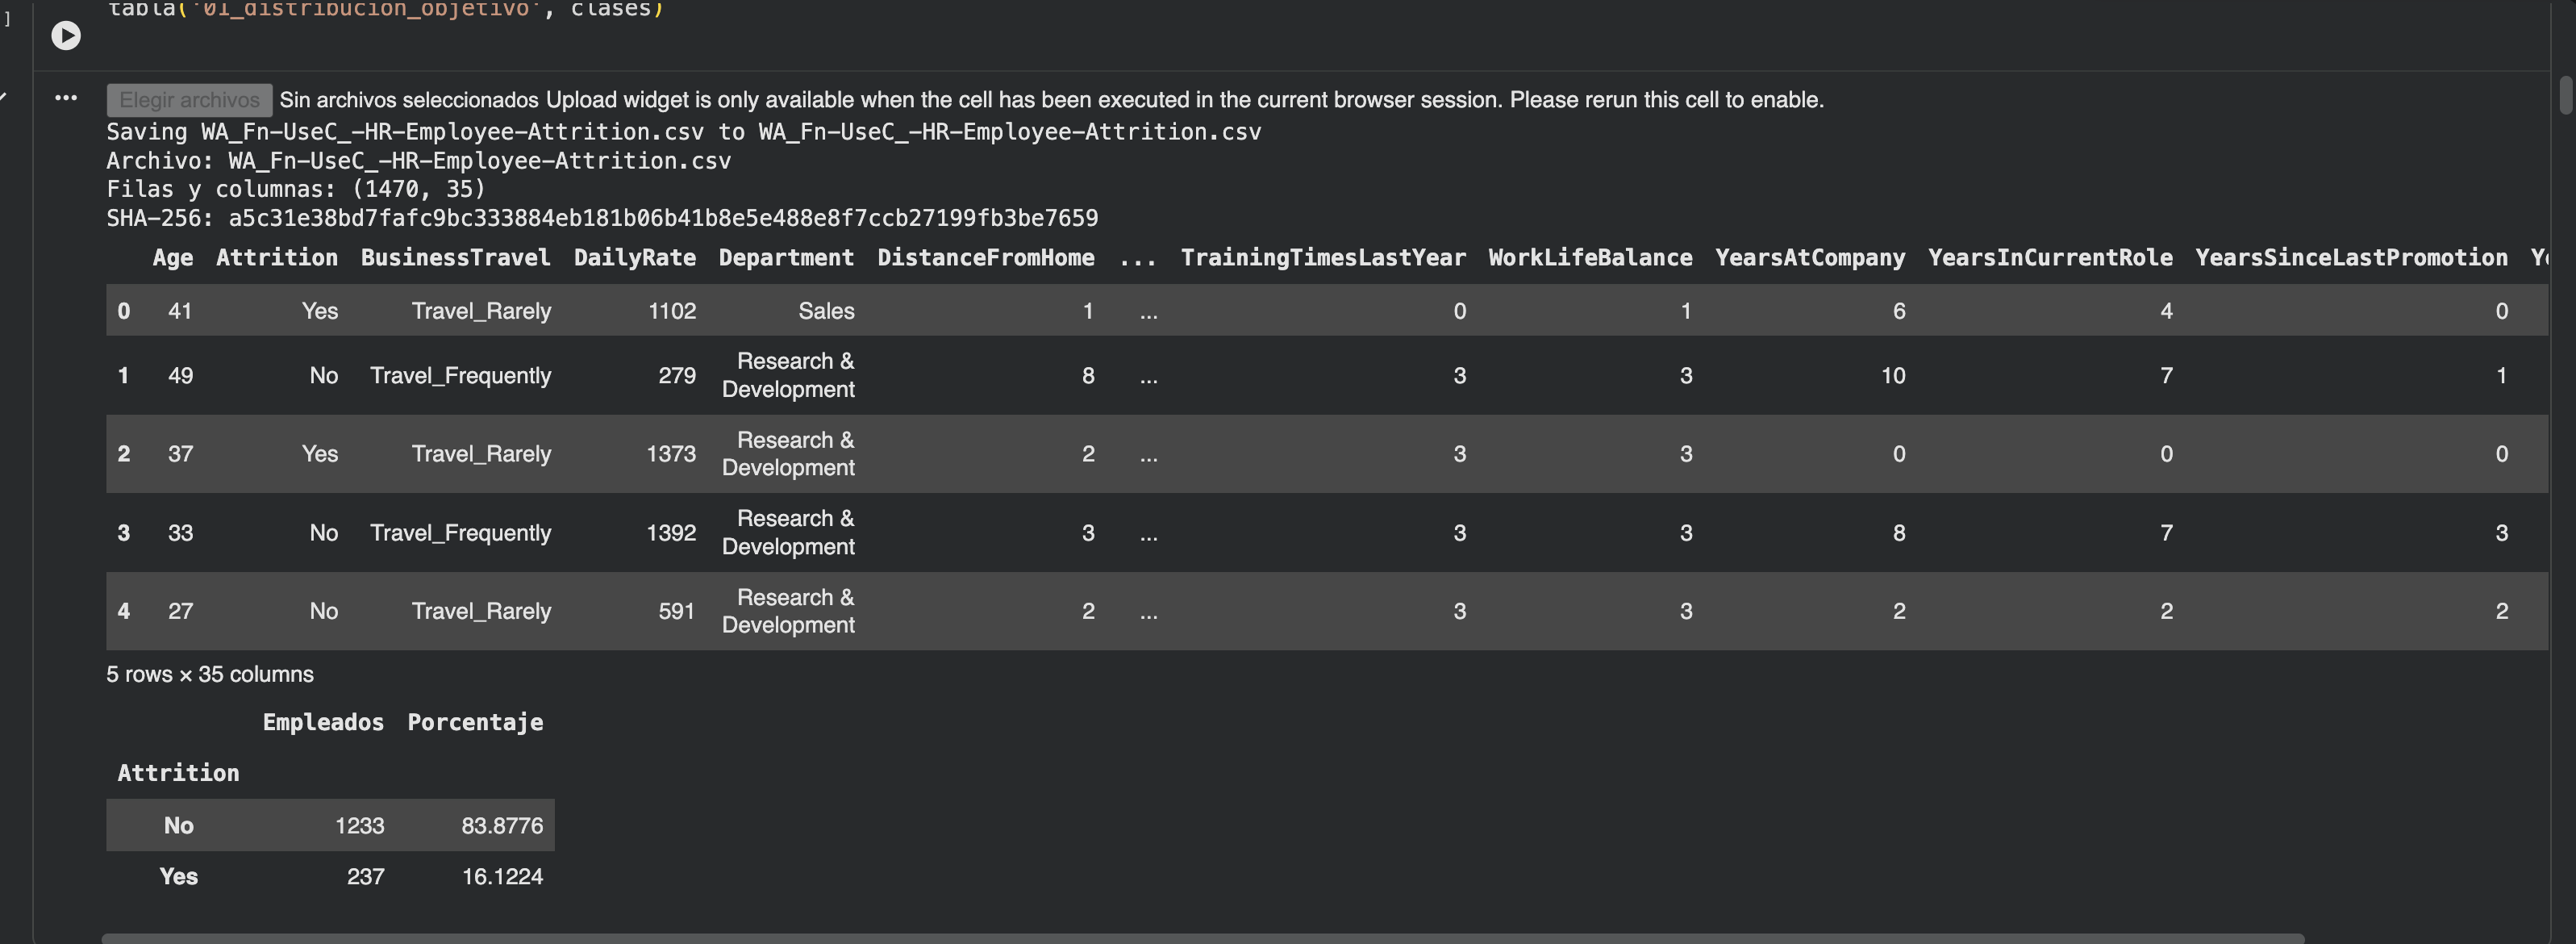
\includegraphics[width=\linewidth,height=0.78\textheight,keepaspectratio]{img/image1.png}
\caption{Carga del archivo, primeros registros y distribucion de Attrition.}
\label{fig:carga-datos}
\end{figure}

\section{Analisis estadistico inicial}
\subsection*{2.1. Tablas dinamicas y cubo de informacion}
\addcontentsline{toc}{subsection}{2.1. Tablas dinamicas y cubo de informacion}
Para esto se uso Attrition con OverTime, Department y JobRole, lo que nos arroja tres tablas con lo satributos de:

-Permanencias.

-Bajas.

-Tamaño de cada grupo.

Ademas de esto se agrego una seccion que combina departamento y horas extra. En cada caso se calcula la tasa de bajas, esto porque comparar solamente los conteos podria hacer que un departamento pareciera tener mas riesgo. Ademas se genero un cubo por departamento y
horas extra.

\[\text{Tasa de bajas (\%)}=100\,\frac{\text{Yes}}{\text{Total}}.\]

\begin{figure}[H]
\centering
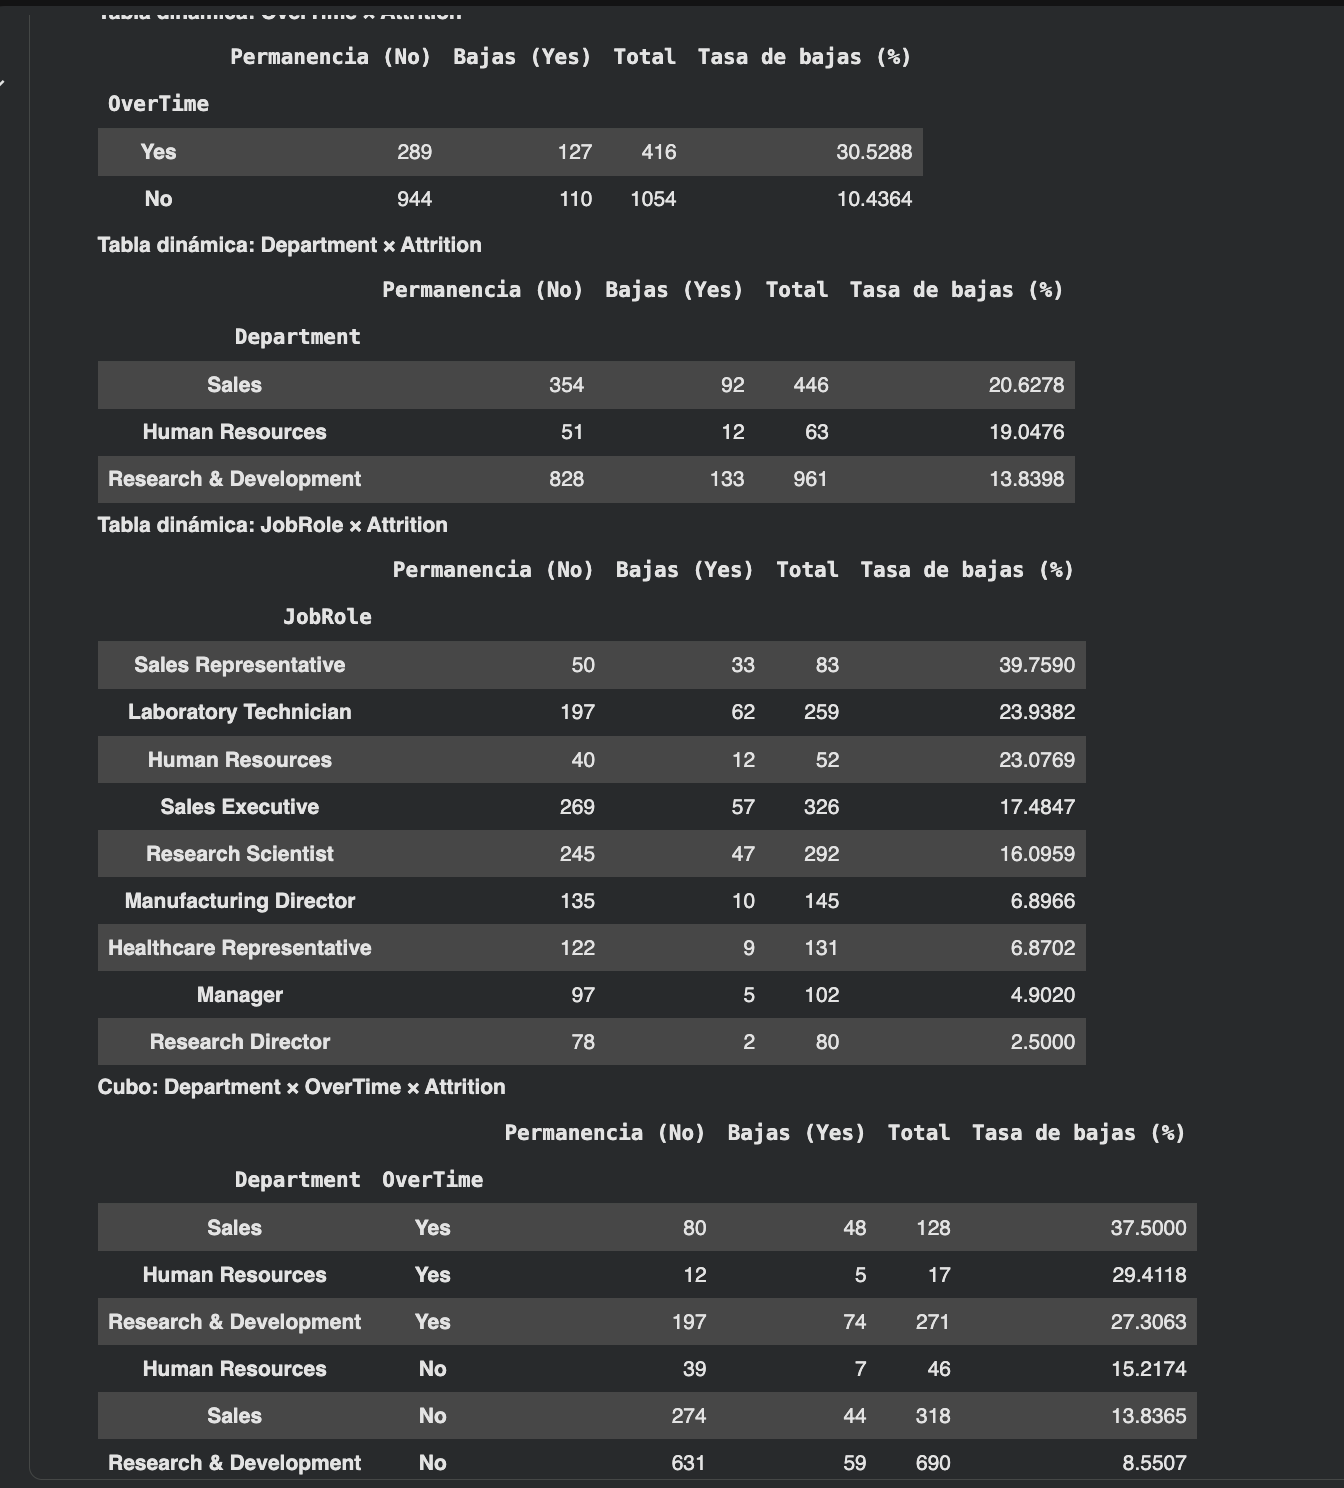
\includegraphics[width=\linewidth,height=0.78\textheight,keepaspectratio]{img/image2.png}
\caption{Tablas dinamicas y cubo por departamento y horas extra.}
\label{fig:tablas-dinamicas}
\end{figure}

En el caso de horas extra, tenemos que una tasa de 30.53\% contra a una tasa de 10.44\% sin horas extra. En el caso de los departamentos, Sales llega con un 20.63\%, mientras que Research \& Development tiene 13.84\%. Por puesto, Sales Representative tiene un 39.76\%, no obstante, este solo tiene untotoal de 83 empleados. Po lo tanto, tanto el tamaño como la tasa se deben de analizar juntos para poder interpretar la comparacion.

\subsection*{Estadistica descriptiva por clase}
\addcontentsline{toc}{subsection}{Estadistica descriptiva por clase}
Despues de esto se obtuvo el promedio, minimo, maximo, desviacion estandar y cuartiles de todas las columnas numericas. Primero se muestran los resultados generales y despues se separan por Attrition, para ver como cambia la distribucion entre bajas y permanencias. En el caso de EmployeeNumber, el calculo se conserva en la salida completa, pero este en si, no se interpreta como una medida del trabajo, esto por que es un identificador. El csv
no dice en si cual es la moneda de ingreso, por lo que se conservan sus valores sin atribuirles pesos
mexicanos o alguna otra moneda.

\begin{table}[H]
\centering
\footnotesize
\setlength{\tabcolsep}{5pt}
\caption{Distribucion por clase de variables utilizadas en la interpretacion.}
\label{tab:grupo}
\begin{tabular}{lrrrrrr}
\toprule
Variable & Clase & Promedio & Desv. est. & Q1 & Mediana & Q3 \\
\midrule
Age & No & 37.56 & 8.89 & 31.00 & 36.00 & 43.00 \\
Age & Yes & 33.61 & 9.69 & 28.00 & 32.00 & 39.00 \\
MonthlyIncome & No & 6,832.74 & 4,818.21 & 3,211.00 & 5,204.00 & 8,834.00 \\
MonthlyIncome & Yes & 4,787.09 & 3,640.21 & 2,373.00 & 3,202.00 & 5,916.00 \\
YearsAtCompany & No & 7.37 & 6.10 & 3.00 & 6.00 & 10.00 \\
YearsAtCompany & Yes & 5.13 & 5.95 & 1.00 & 3.00 & 7.00 \\
TotalWorkingYears & No & 11.86 & 7.76 & 6.00 & 10.00 & 16.00 \\
TotalWorkingYears & Yes & 8.24 & 7.17 & 3.00 & 7.00 & 10.00 \\
DistanceFromHome & No & 8.92 & 8.01 & 2.00 & 7.00 & 13.00 \\
DistanceFromHome & Yes & 10.63 & 8.45 & 3.00 & 9.00 & 17.00 \\
JobSatisfaction & No & 2.78 & 1.09 & 2.00 & 3.00 & 4.00 \\
JobSatisfaction & Yes & 2.47 & 1.12 & 1.00 & 3.00 & 3.00 \\
\bottomrule
\end{tabular}
\end{table}

\begin{figure}[H]
\centering
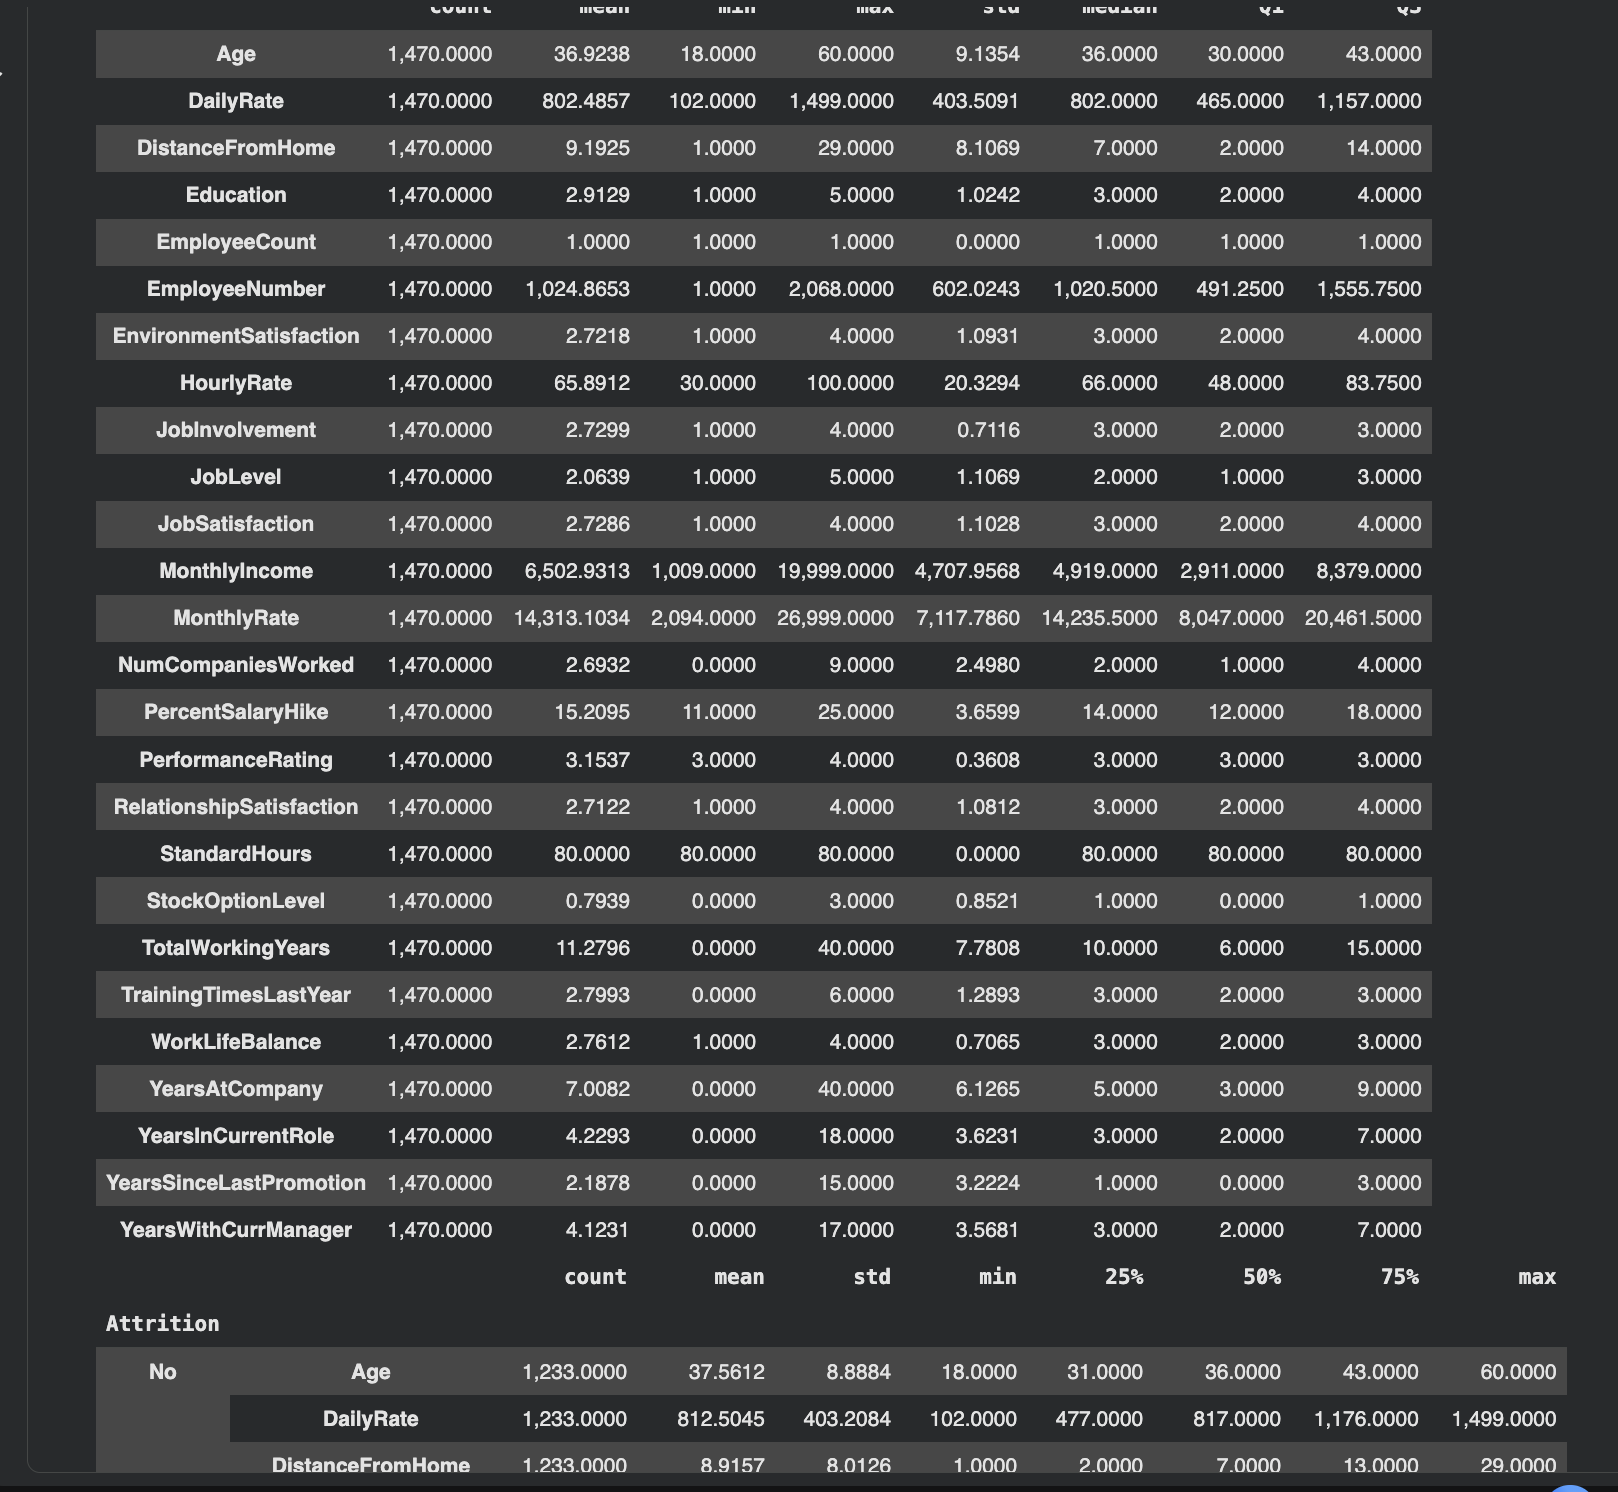
\includegraphics[width=\linewidth,height=0.78\textheight,keepaspectratio]{img/image3.png}
\caption{Salida de las estadisticas descriptivas generales y por clase.}
\label{fig:estadisticas}
\end{figure}

\subsection*{Graficas comparativas}
\addcontentsline{toc}{subsection}{Graficas comparativas}
Ahora bien, para revisar los resultados de las tabblas se graficaron las tasas de bajas por horas extra y departamento. Tambien se compararon los ingresos y la antigüedad mediante diagramas de caja. La linea central
indica la mediana y la caja reune el 50\% central de los registros, los puntos extremos requieren
contexto.

\begin{figure}[H]
\centering
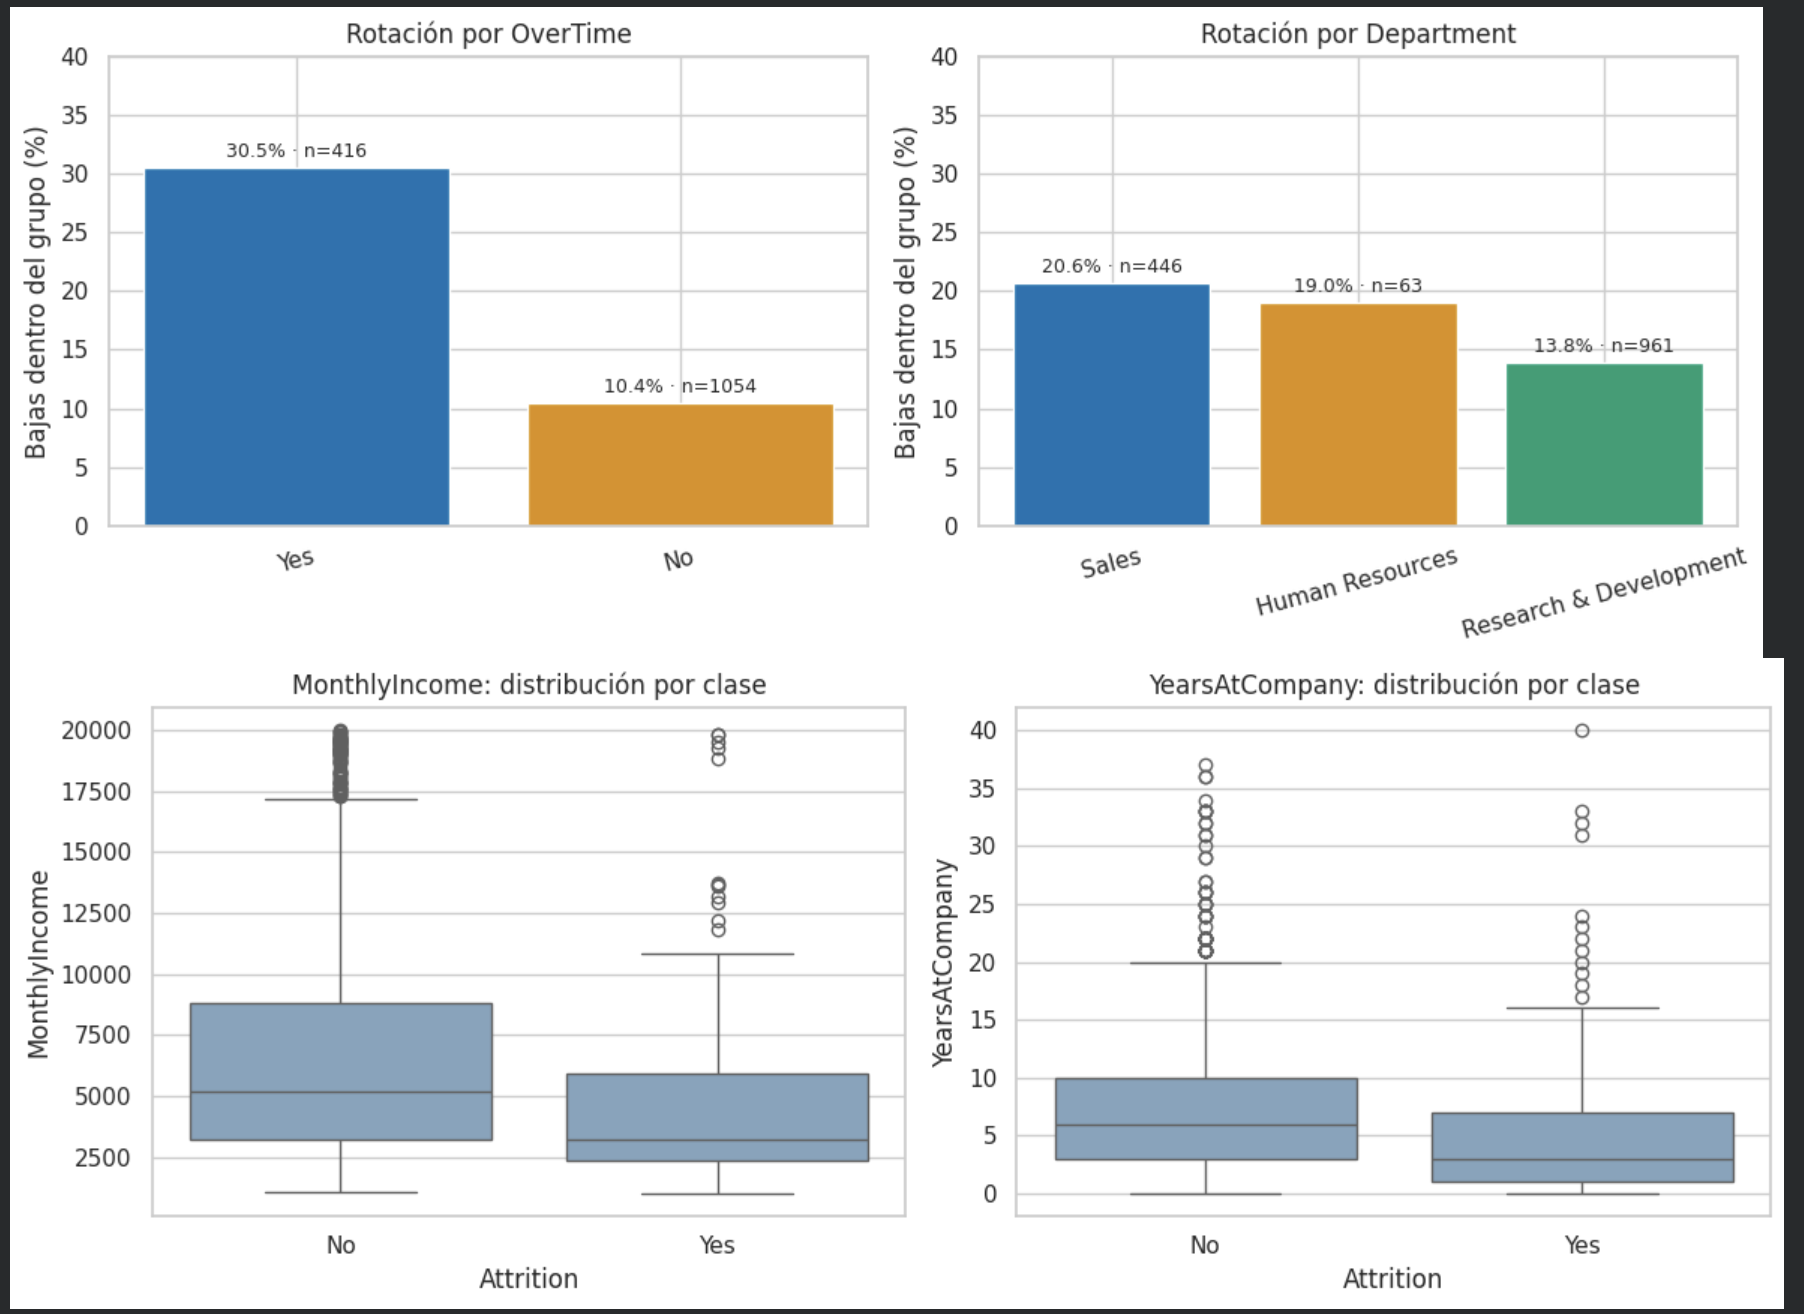
\includegraphics[width=\linewidth,height=0.78\textheight,keepaspectratio]{img/image4.png}
\caption{Tasas de bajas, ingreso mensual y antiguedad por clase.}
\label{fig:graficas-eda}
\end{figure}

Interpretacion:

La primera parte nos dice que 237 bajas de 1470 empleados lo que es un 16.1\%, por lo que tenemos una clase minoritaria.

Ahora bien, con horas extra la tasa de bajas es 30.5\%, frente a 10.4\% sin horas extra.

Sales es el departamento con mayor tasa, la cual tiene un 20.6\%, por lo que también hay que revisar cuántos empleados contiene.

Sales Representative es el puesto con mayor tasa (39.8\%, n=83).

Al comparar ingresos, el promedio es 4,787.09 en bajas y 6,832.74 en permanencias, aqui tenemos un problema, debido a que el archiv no indica la unidad monetaria.

En el caso de la antigüedad, la media es 5.13 años en bajas y 7.37 en permanencias.

\#\#Lo que se tieen aqui es una relacion con carga laboral, remuneracion y trayectoria, para comprobar el efecto de un cambio se necesitaria otro analisis.

\section{EDA y preparacion de variables}

Para esto se reviso cada columna con conteo de nulos, tipo de dato, categorias y cantidad de valores
diferentes.

Se logro identificar 26 columnas almacenadas como enteros y nueve como texto, con esto despues de separar la etiqueta y retirar las cuatro descartadas quedan 23 columnas numericas y siete nominales.

Ademas se reviso que la edad estuviera entre 18 y 100 años, que el ingreso mensual fuera positivo y que los años en la empresa no superaran la experiencia total.

Se compararon tambien años en el puesto, con el gerente y desde la promocion contra los años en la empresa, y las cinco escalas de satisfaccion o participacion contra el rango de 1 a 4. Las once reglas arrojaron cero casos para revisar.

Las edades que se tienen van de 18 a 60 años y los valores extremos se conservaron.

\begin{figure}[H]
\centering
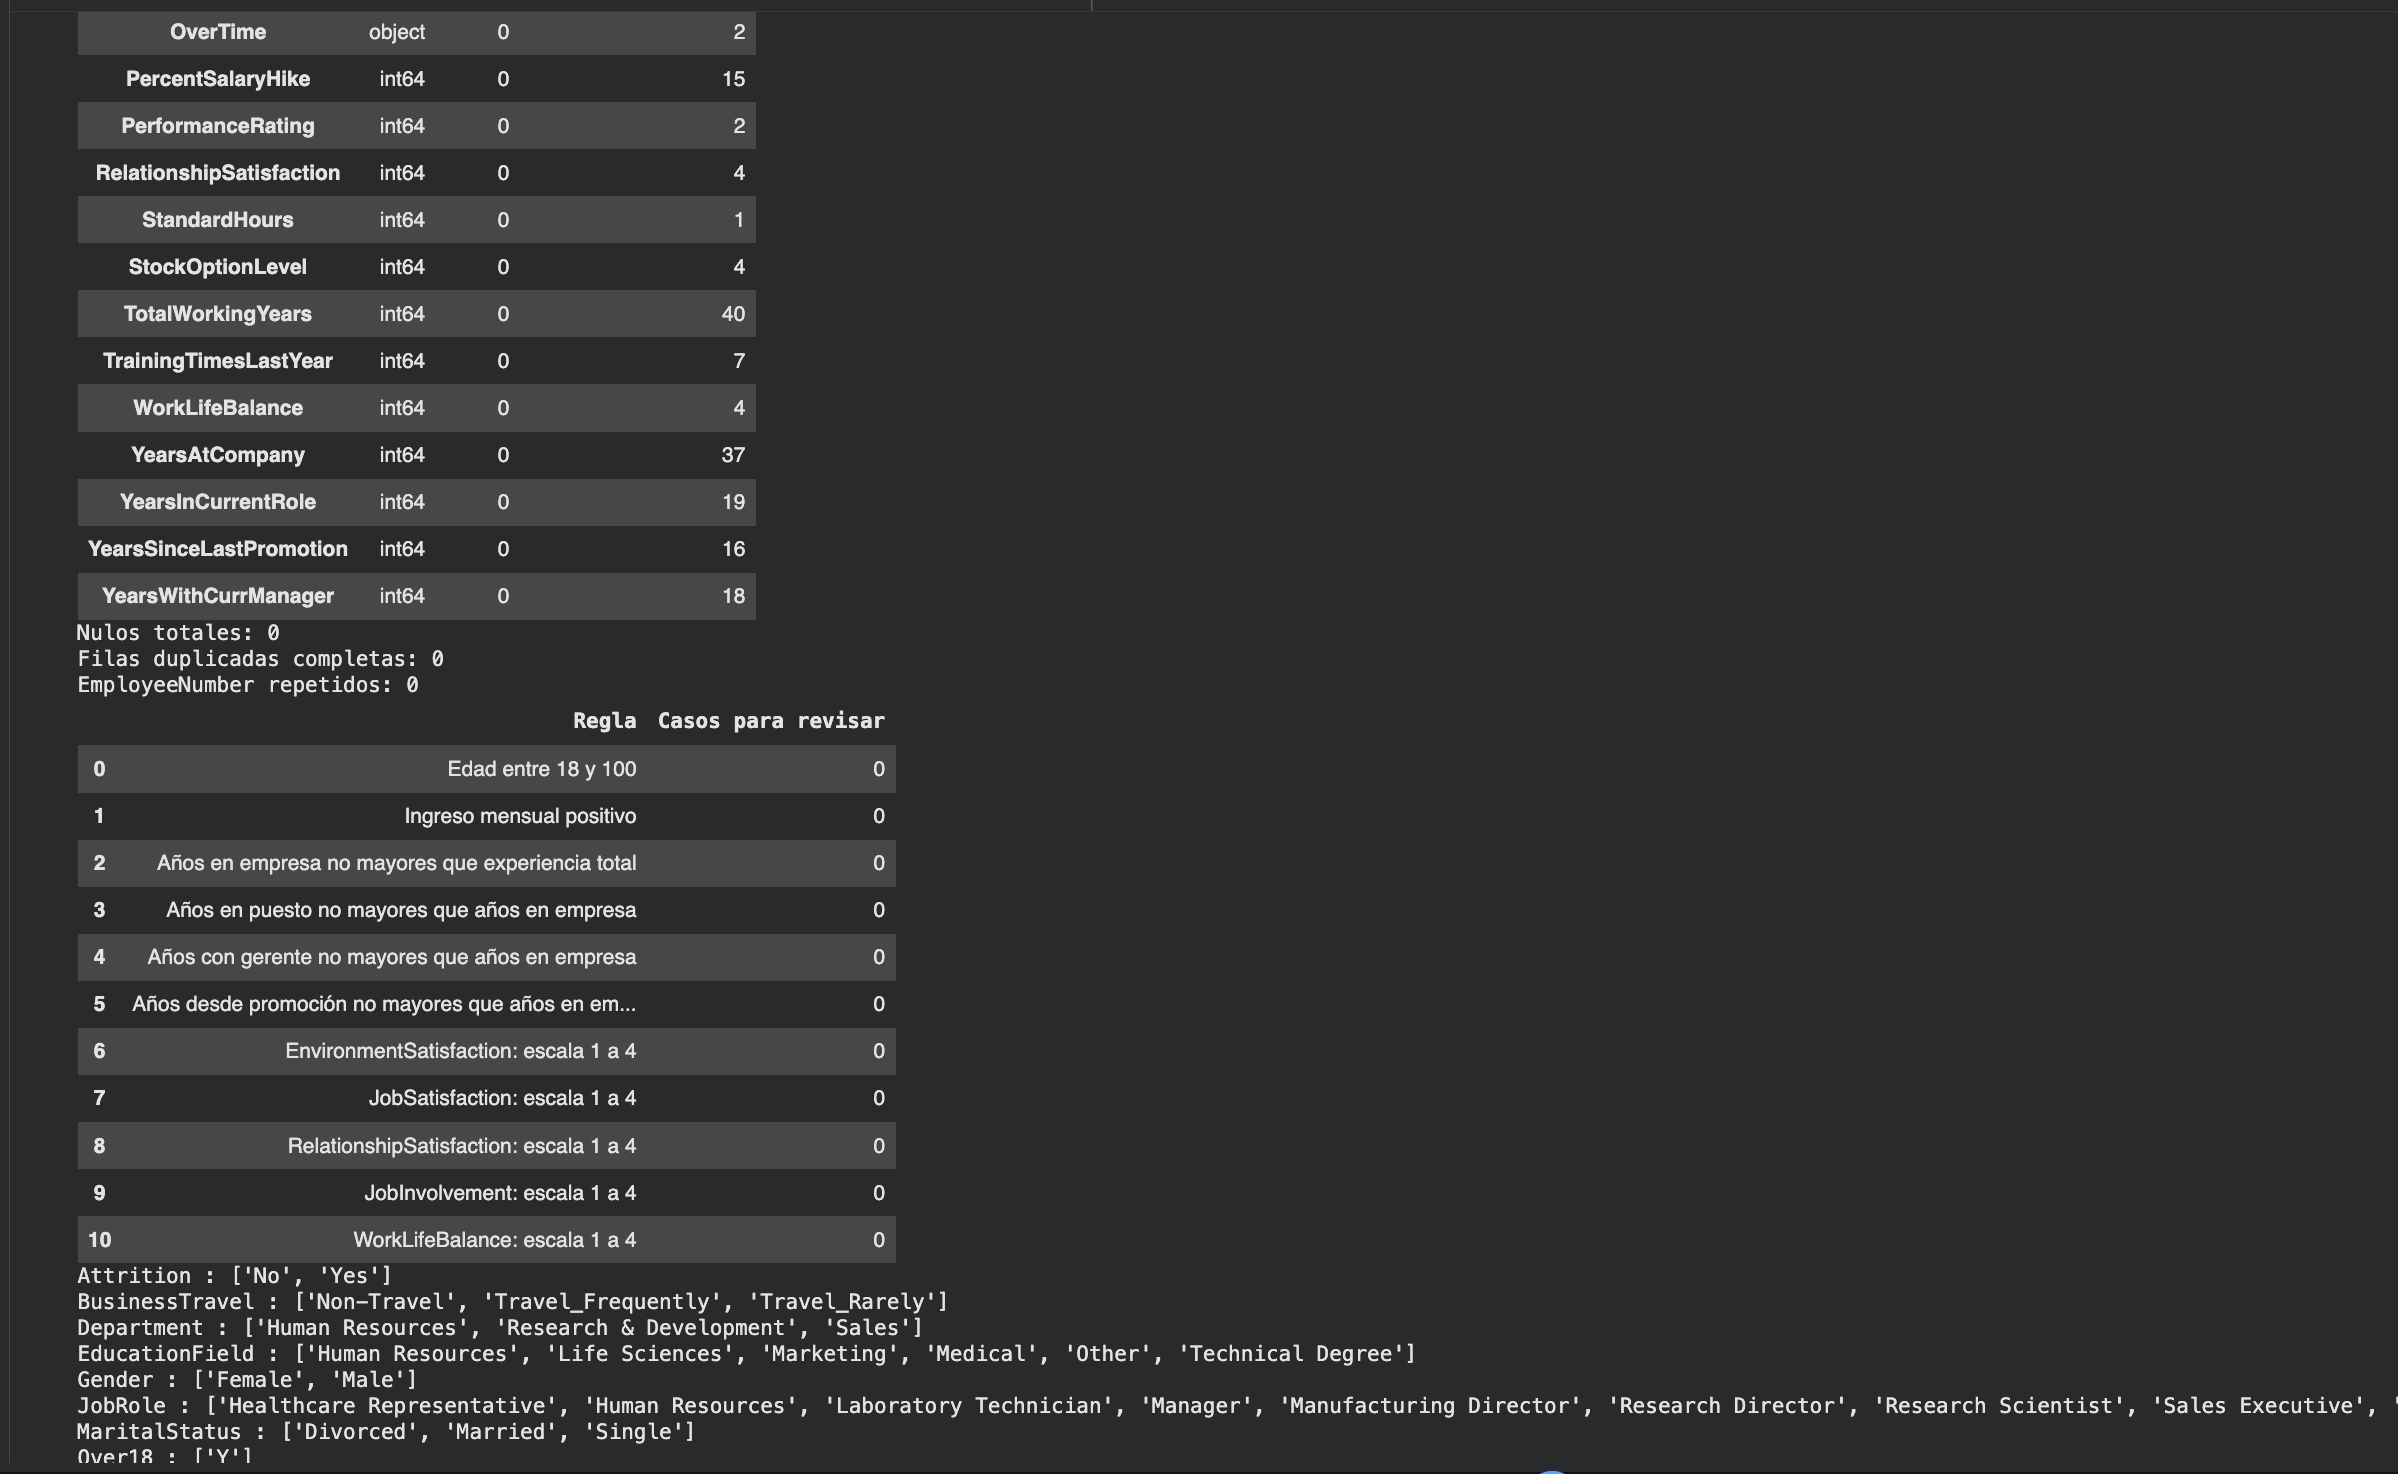
\includegraphics[width=\linewidth,height=0.78\textheight,keepaspectratio]{img/image5.png}
\caption{Revision de nulos, duplicados, reglas de consistencia y categorias.}
\label{fig:calidad-datos}
\end{figure}

\subsection*{Variables seleccionadas y descartadas}
\addcontentsline{toc}{subsection}{Variables seleccionadas y descartadas}
Se utilizaron 30 predictores, donde se incluyen condiciones del puesto, satisfaccion, compensacion, formacion y trayectoria. La razon por la que se conservaron es que permiten revisar distintas condiciones laborales y comparar los cinco modelos con la misma informacion.

En el caso de EmployeeNumber, se descarto porque identifica al empleado. Tambien se retiraron EmployeeCount, Over18 y StandardHours, porque tienen un mismo valor en todas las filas. Attrition se separo como etiqueta. Las escalas de satisfaccion y nivel se mantuvieron como numeros ordinales, lo que supone una distancia igual entre niveles, las categorias sin orden se convierten con one-hot.

Cabe mencionar que Gender, Age y MaritalStatus se conservan para esta comparacion, pero se necesita revisar si se es que llegaran a tener sesgos. Esto por que, que una columna ayude a predecir no significa que sea adecuada para decidir sobre una persona. Por esto se agrego una parte por genero y se propone comparar despues una version sin estos atributos.

\begin{figure}[H]
\centering
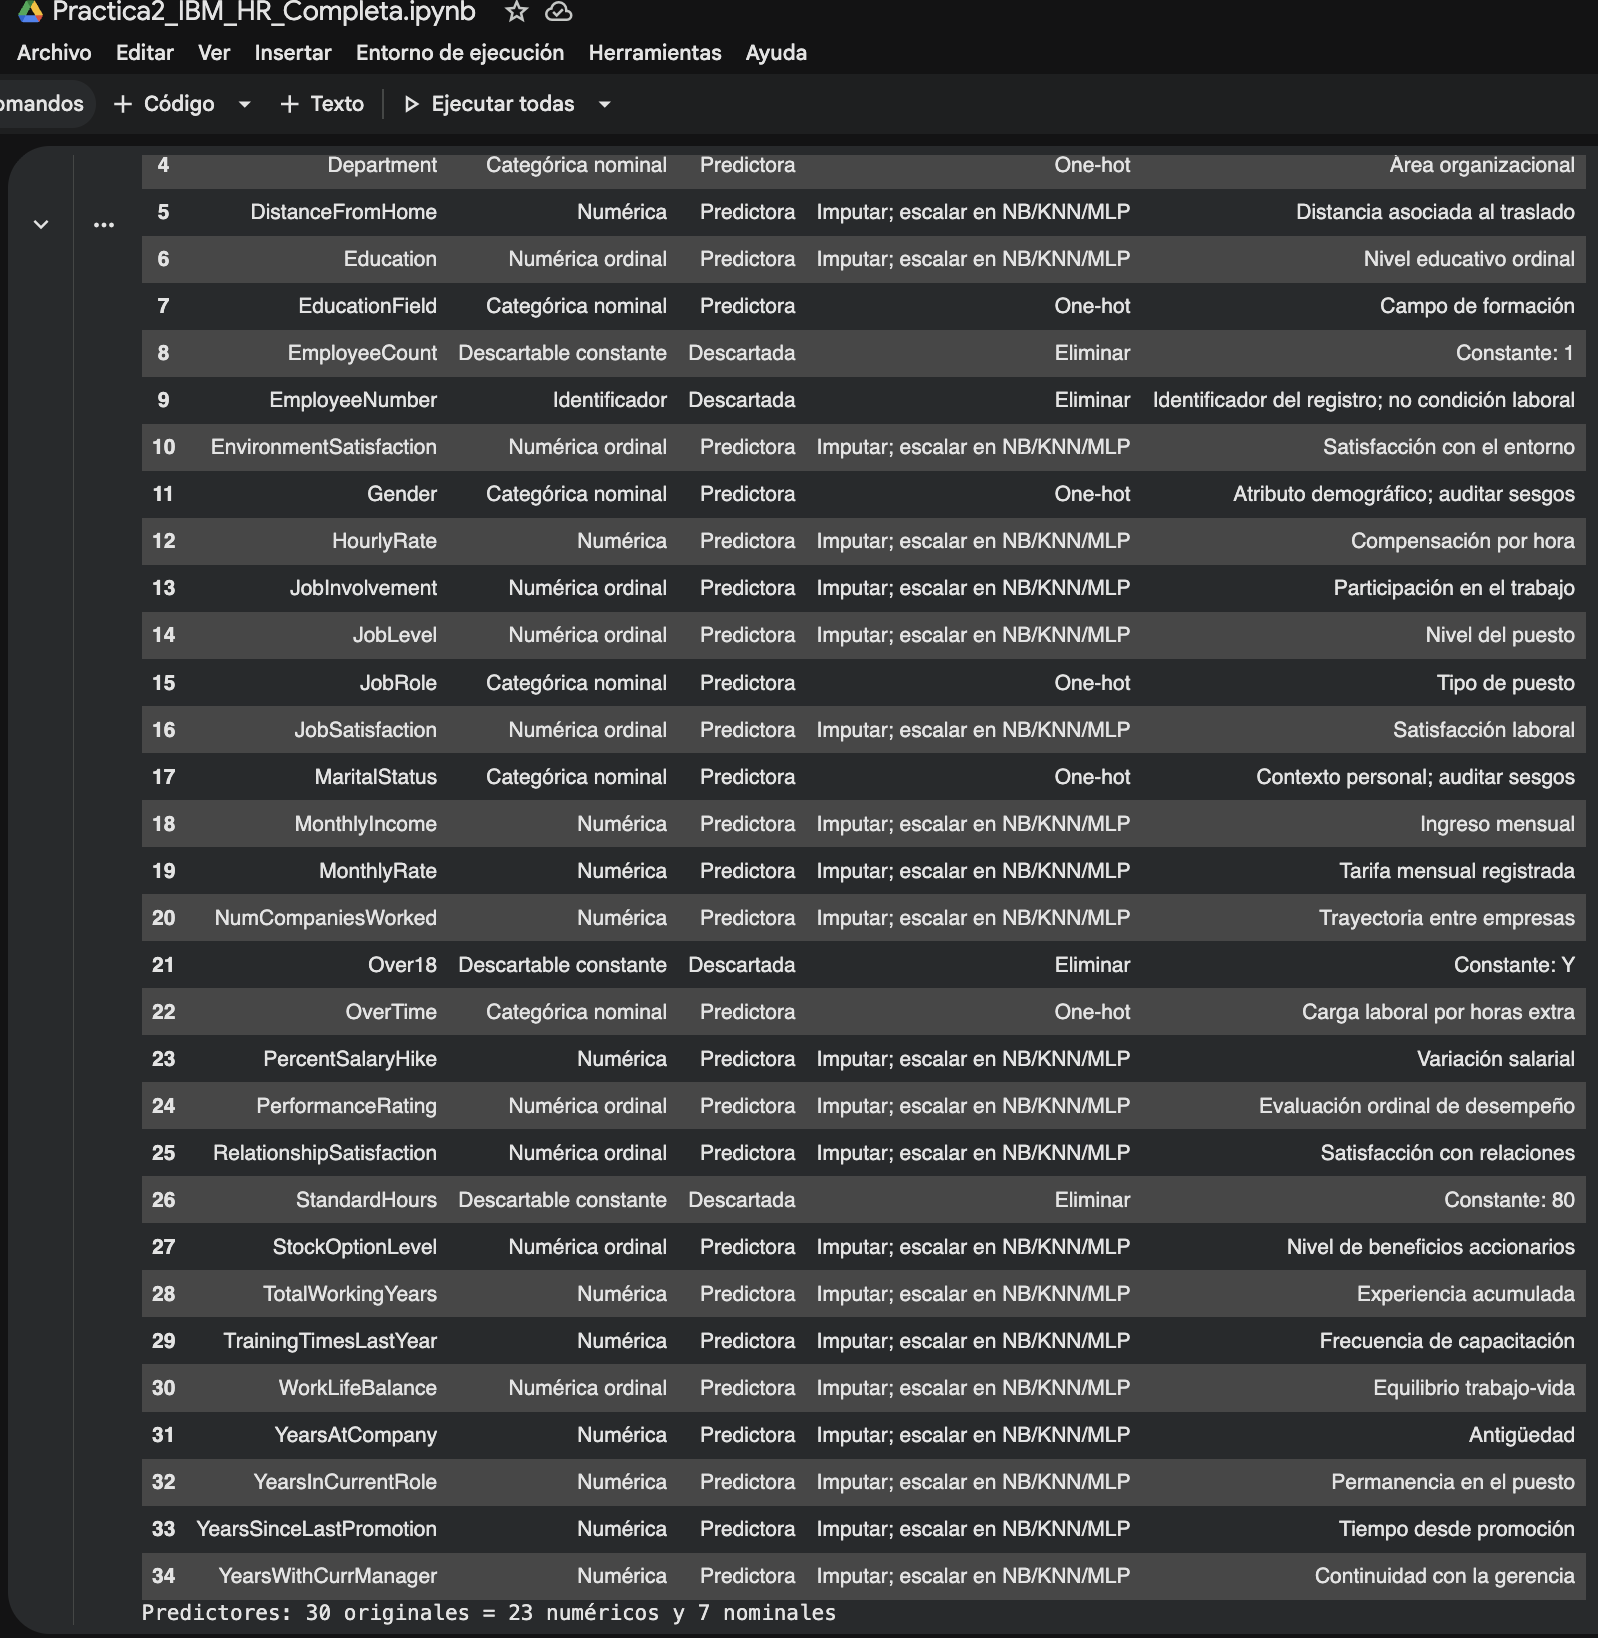
\includegraphics[width=\linewidth,height=0.6\textheight,keepaspectratio]{img/image6.png}
\caption{Clasificacion, seleccion y descarte de las variables.}
\label{fig:seleccion-variables}
\end{figure}

\subsection*{Transformacion de las variables}
\addcontentsline{toc}{subsection}{Transformacion de las variables}
Primero se separan los datos y despues se ajustan las transformaciones dentro de entrenamiento. Para esto se utilizaron Pipeline y ColumnTransformer, de manera que en cada fold la mediana, el escalado y las categorias se aprenden solamente con las filas que se usan para entrenar. En prueba se aplica la transformacion que ya quedo ajustada.

Las columnas numericas se atribuye a la mediana y se escalan con StandardScaler para NB, KNN y la red neuronal. Las nominales son parte, ahora con la moda y se convierten con OneHotEncoder.

Actualmente no hay nulos, pero se deja que hacer si aparecen. En el arbol y Random Forest se conservan las unidades originales de las numericas, para que sus cortes se puedan leer con mayor facilidad.

Las siete nominales generan 28 indicadores: viajes (3), departamento (3), formacion (6), genero (2), puesto (9), estado civil (3) y horas extra (2). Junto con las 23 numericas se tienen 51 entradas transformadas.

\begin{figure}[H]
\centering
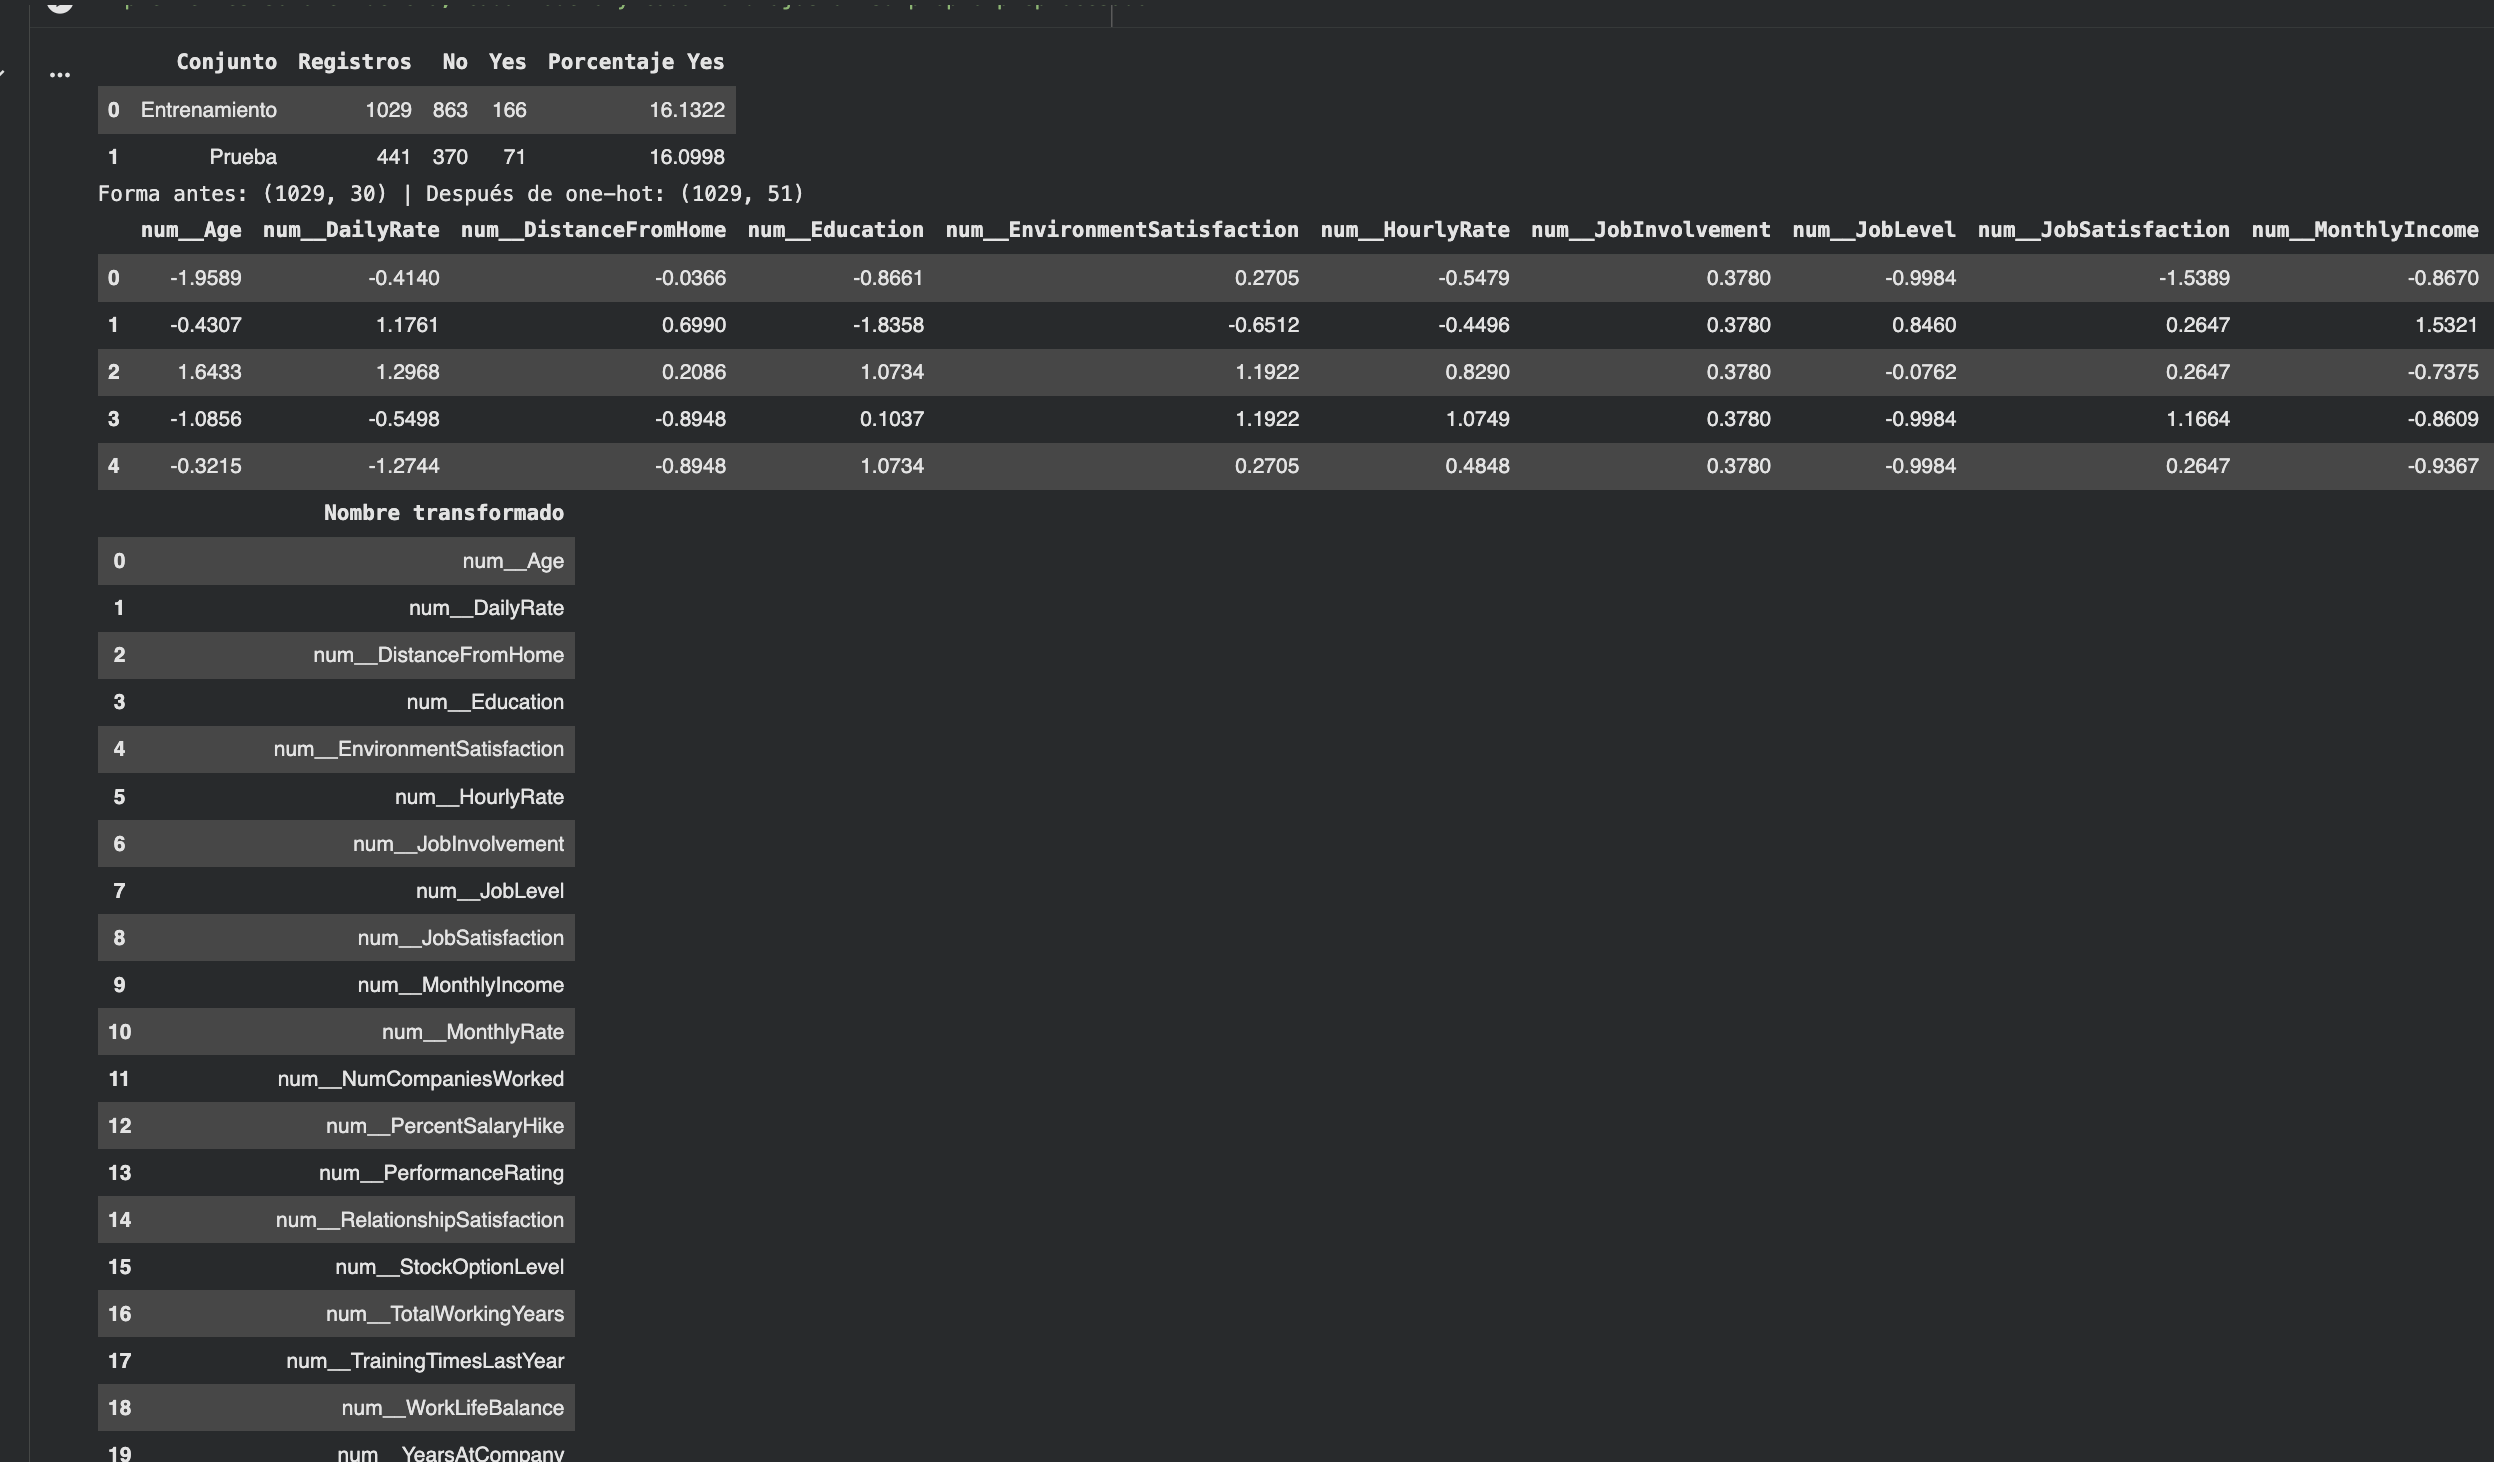
\includegraphics[width=\linewidth,height=0.78\textheight,keepaspectratio]{img/image7.png}
\caption{Particion y resultado de la transformacion de los predictores.}
\label{fig:transformaciones}
\end{figure}

Para esto, la primera tabla nos muestra la base en los conjuntos de entrenamiento y prueba.
Ahora bien, el conjunto de entrenamiento quedo teniendo por 1029 registros y el de prueba por 441.
En el caso de entrenamiento la tasa de rotación es de 16.13\%, mientras que en prueba se tiene un 16.09\%.
Se pasó de tener 30 columnas originales a 51 atributos finales debido a la codificación one-hot de las nominales.

Finalmente, los valores resultantes muestran decimales, confirmando que el escalado se hizo correctamente.

\section{Aplicación de primeros modelos de Machine Learning}

\subsection*{4.1. División de datos en entrenamiento y prueba}
\addcontentsline{toc}{subsection}{4.1. División de datos en entrenamiento y prueba}

Para esto se utilizó una partición estratificada de 70/30, donde quedaron 1,029 registros para entrenamiento y 441 para prueba.

\begin{figure}[H]
\centering
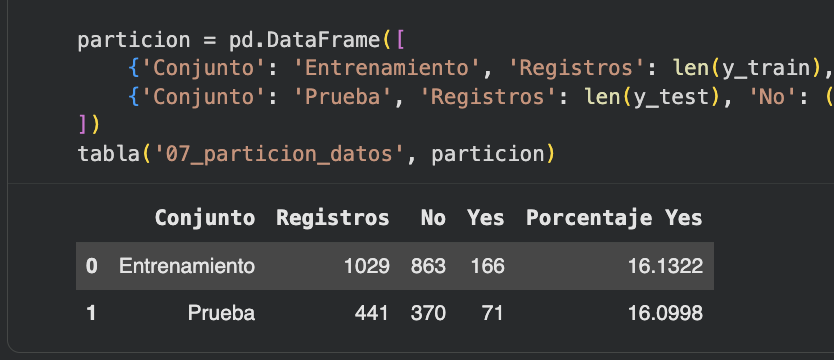
\includegraphics[width=\linewidth,height=0.78\textheight,keepaspectratio]{img/image8.png}
\caption{Distribucion de las clases en entrenamiento y prueba.}
\label{fig:particion}
\end{figure}

\subsection*{4.2. Entrenamiento y configuración de modelos}
\addcontentsline{toc}{subsection}{4.2. Entrenamiento y configuración de modelos}

Dentro de entrenamiento se compararon unas cuantas configuraciones mediante tres folds estratificados. Se eligió F1 de Yes como criterio principal y se conservó el umbral de 0.5. Posteriormente, la mejor configuración de cada modelo se ajustó con todo entrenamiento y se evaluó en la prueba reservada.

\begin{table}[H]
\centering\footnotesize
\begin{tabularx}{\linewidth}{L{3.0cm}YY}
\toprule
Modelo & Qué hace & Preparación y configuración revisada \\
\midrule
Naive Bayes gaussiano & Estima distribuciones por clase & Escalado y suavizado de varianza; one-hot aproxima entradas gaussianas \\
K-Nearest Neighbor & Compara vecinos por distancia & Escalado, k=5/11 y voto por distancia \\
Árbol de decisión & Genera reglas mediante cortes & Profundidad 3/5, mínimo 10 por hoja y pesos balanceados \\
Random Forest & Combina 200 árboles & Profundidad limitada o libre, mínimo por hoja y pesos balanceados opcionales \\
Red neuronal MLP & Aprende relaciones mediante capas & Escalado, capas de 20 y 10 neuronas, regularización L2 y Adam \\
\bottomrule
\end{tabularx}
\end{table}

Además de esto se agregó una referencia que siempre predice No. Lo que nos permite ver es cuánta exactitud se puede obtener por la clase mayoritaria, aun cuando no se detecte ninguna baja. No se modificaron las proporciones de la prueba ni se aplicó sobremuestreo sobre toda la base.

\begin{figure}[H]
\centering
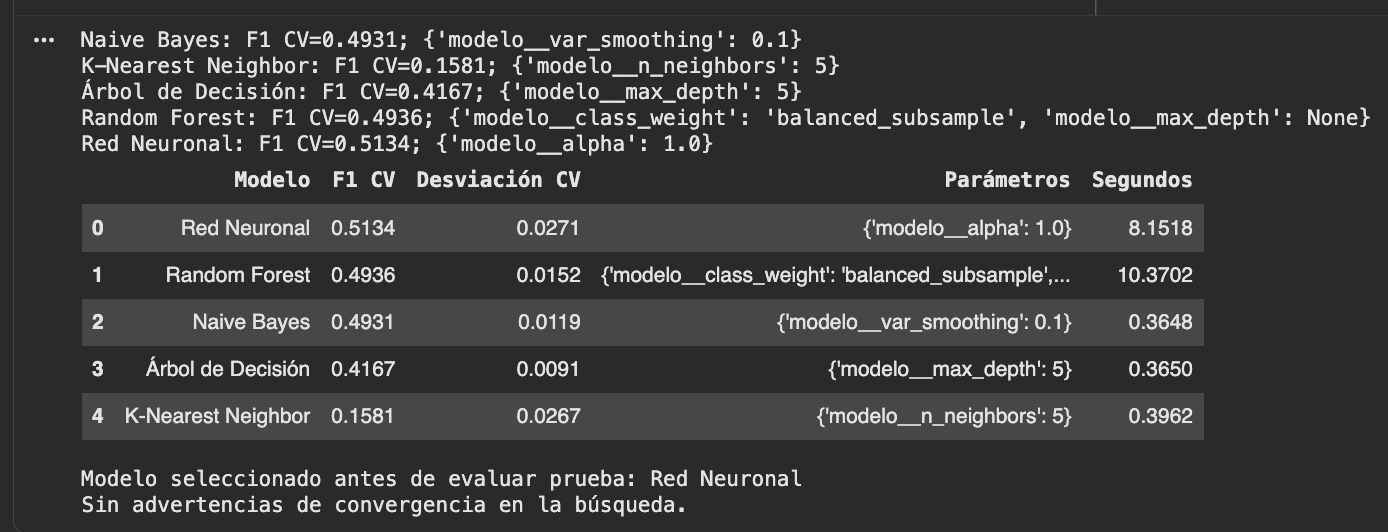
\includegraphics[width=\linewidth,height=0.78\textheight,keepaspectratio]{img/image9.png}
\caption{Entrenamiento, validacion cruzada y configuraciones seleccionadas.}
\label{fig:validacion-cruzada}
\end{figure}

\subsection*{4.3. Evaluación de los modelos}
\addcontentsline{toc}{subsection}{4.3. Evaluación de los modelos}

La exactitud indica cuántas predicciones fueron correctas en total. La precisión de Yes nos dice cuántas alertas sí correspondían a bajas; el recall de Yes, cuántas de las bajas reales se detectaron. F1 reúne precisión y recall. También se calcula ROC-AUC con las probabilidades y AP, que resume la curva precision-recall. El F1 ponderado se deja en la salida adicional para comparar con el ejemplo de la guía.

\[
\text{Precision}=\frac{TP}{TP+FP},\qquad
\mathrm{Recall}=\frac{TP}{TP+FN},\qquad
F1=\frac{2\,\text{Precision}\,\mathrm{Recall}}{\text{Precision}+\mathrm{Recall}}.
\]

\begin{figure}[H]
\centering
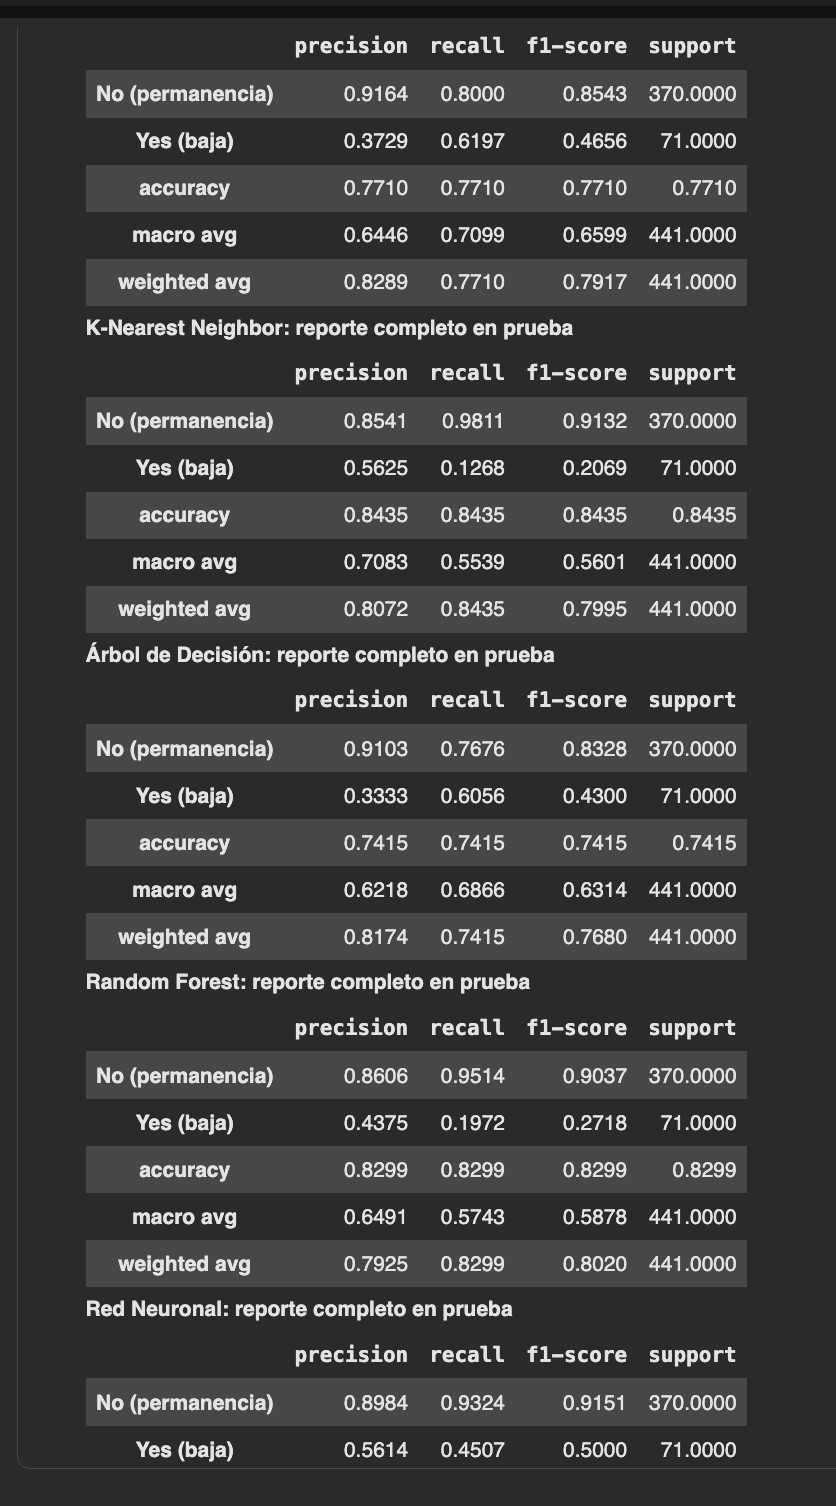
\includegraphics[width=\linewidth,height=0.78\textheight,keepaspectratio]{img/image10.png}
\caption{Reportes de clasificacion de los cinco modelos.}
\label{fig:reportes-clasificacion}
\end{figure}

En las matrices, las filas corresponden a la clase real y las columnas a la predicción: [[TN, FP], [FN, TP]]. En este caso un falso negativo es una baja que no se detectó, mientras que un falso positivo es una alerta sobre un empleado que permaneció.

\begin{figure}[H]
\centering
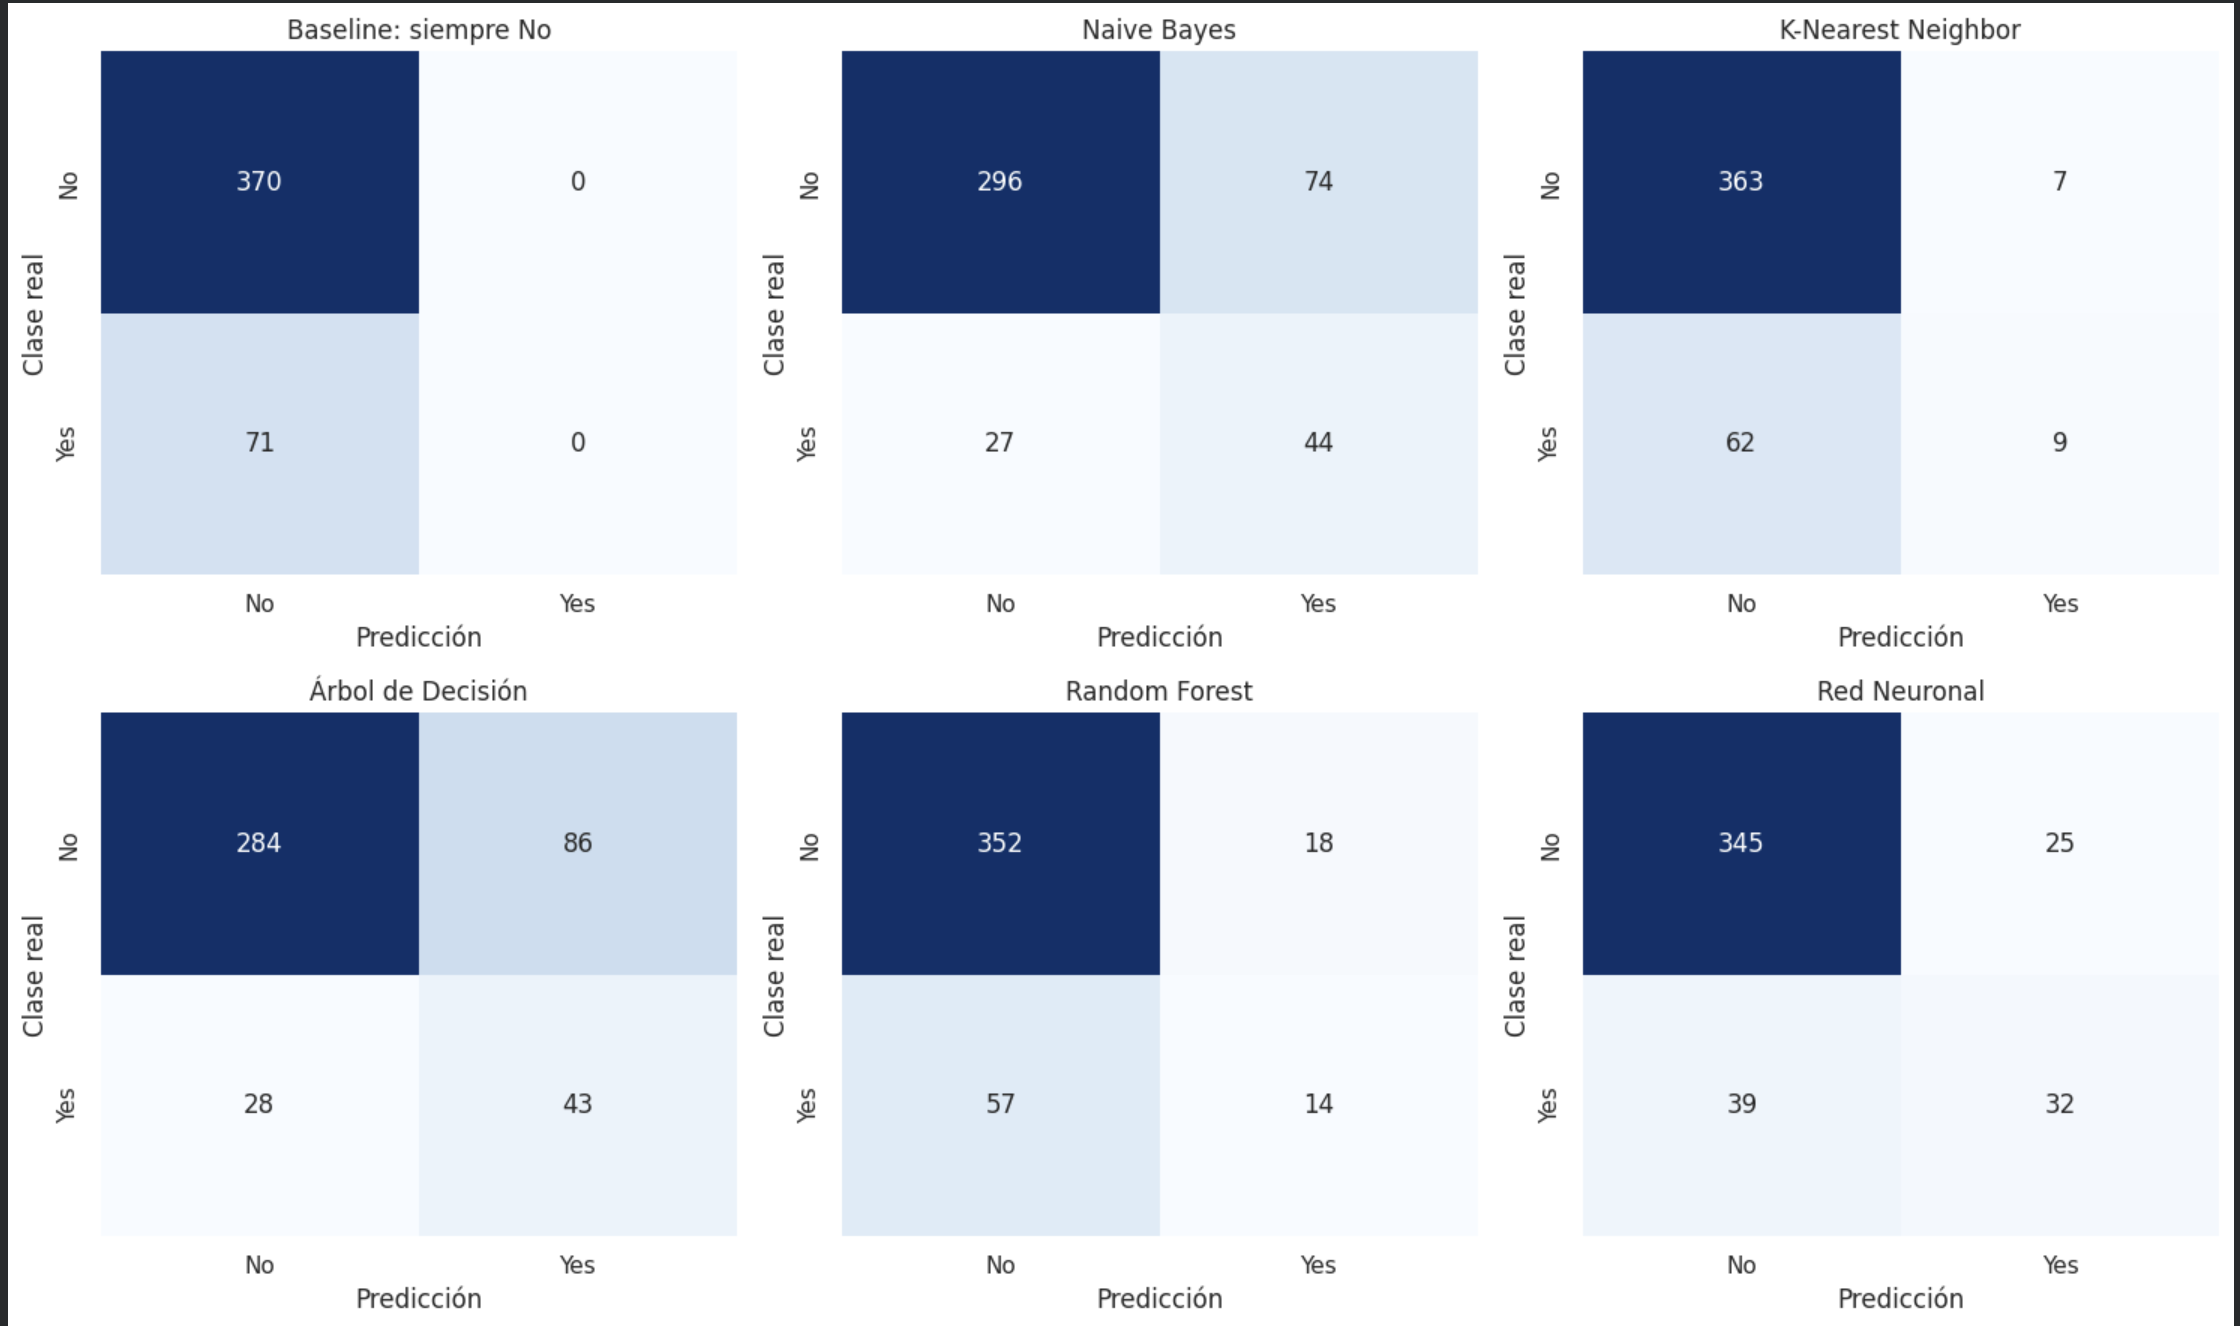
\includegraphics[width=\linewidth,height=0.3\textheight,keepaspectratio]{img/image11.png}
\caption{Matrices de confusion de la referencia y los cinco modelos.}
\label{fig:matrices-confusion}
\end{figure}

Para las curvas se utilizan las probabilidades, porque las etiquetas por sí solas no permiten revisar distintos umbrales. Esto responde a la instrucción de agregar la métrica de ROC o AUC para revisar la capacidad de discriminación del modelo.

\begin{figure}[H]
\centering
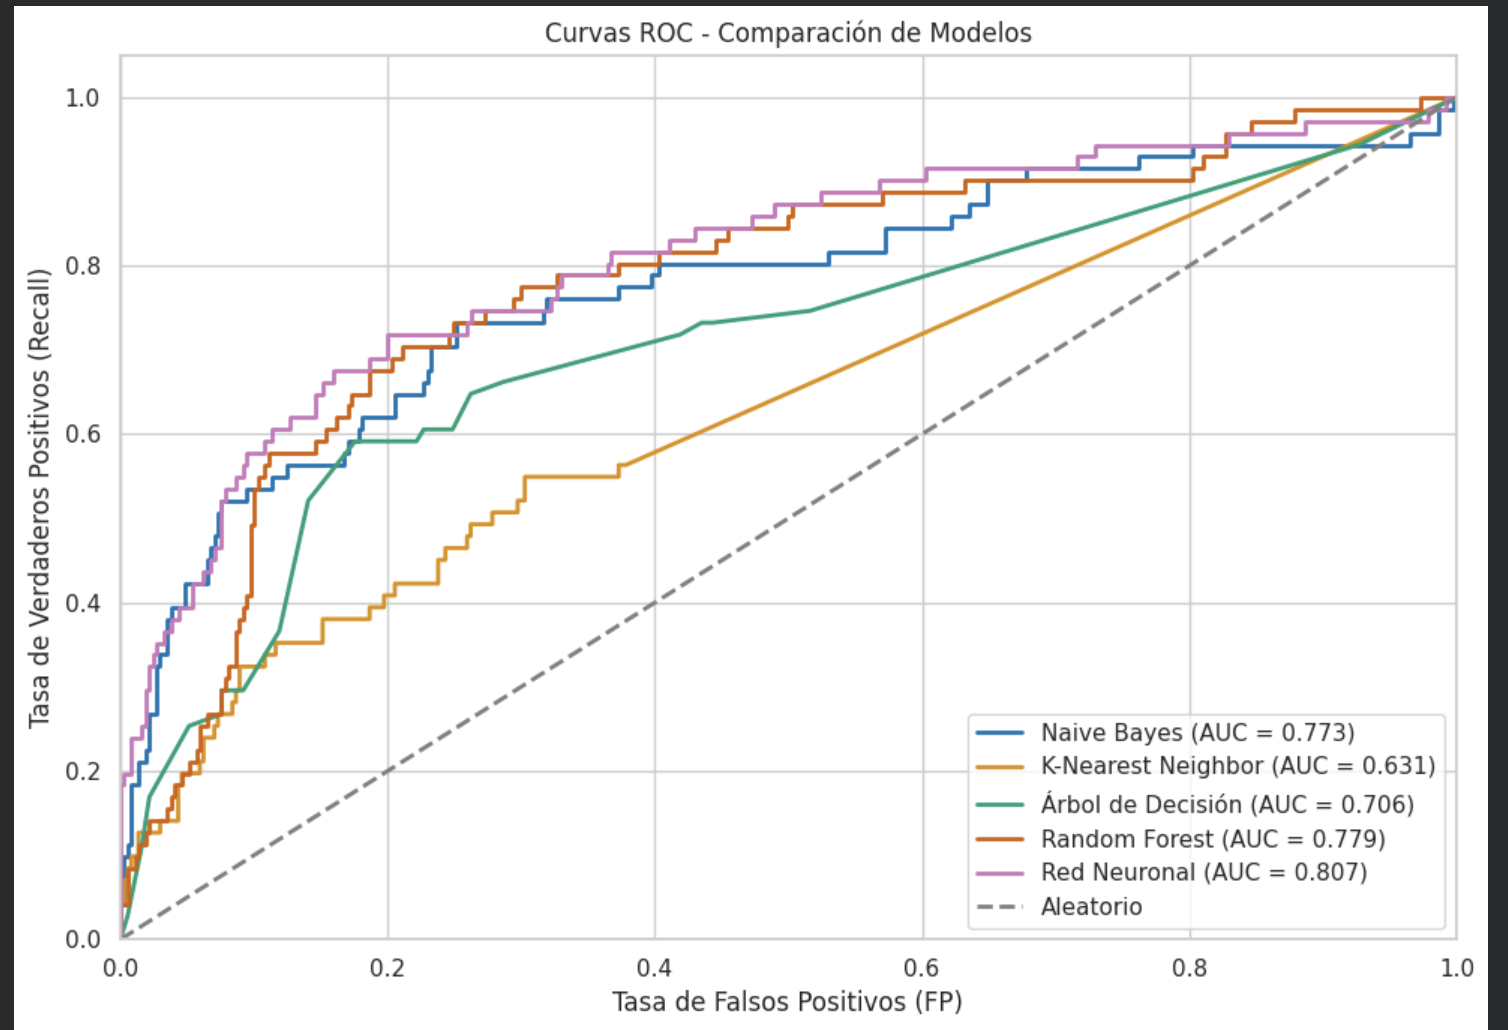
\includegraphics[width=\linewidth,height=0.25\textheight,keepaspectratio]{img/image12.png}
\caption{Curvas ROC obtenidas con las probabilidades de los modelos.}
\label{fig:roc-evaluacion}
\end{figure}

\section{Comparación de modelos}

Ahora bien, el cuadro siguiente reúne exactitud, precisión, recall y F1 de prueba. Las tres últimas métricas corresponden a bajas (Yes), no a un promedio de las clases. En la columna de variables se indican las 30 originales y las transformadas (el conjunto completo se documentó en pasos anteriores).

\begin{figure}[H]
\centering
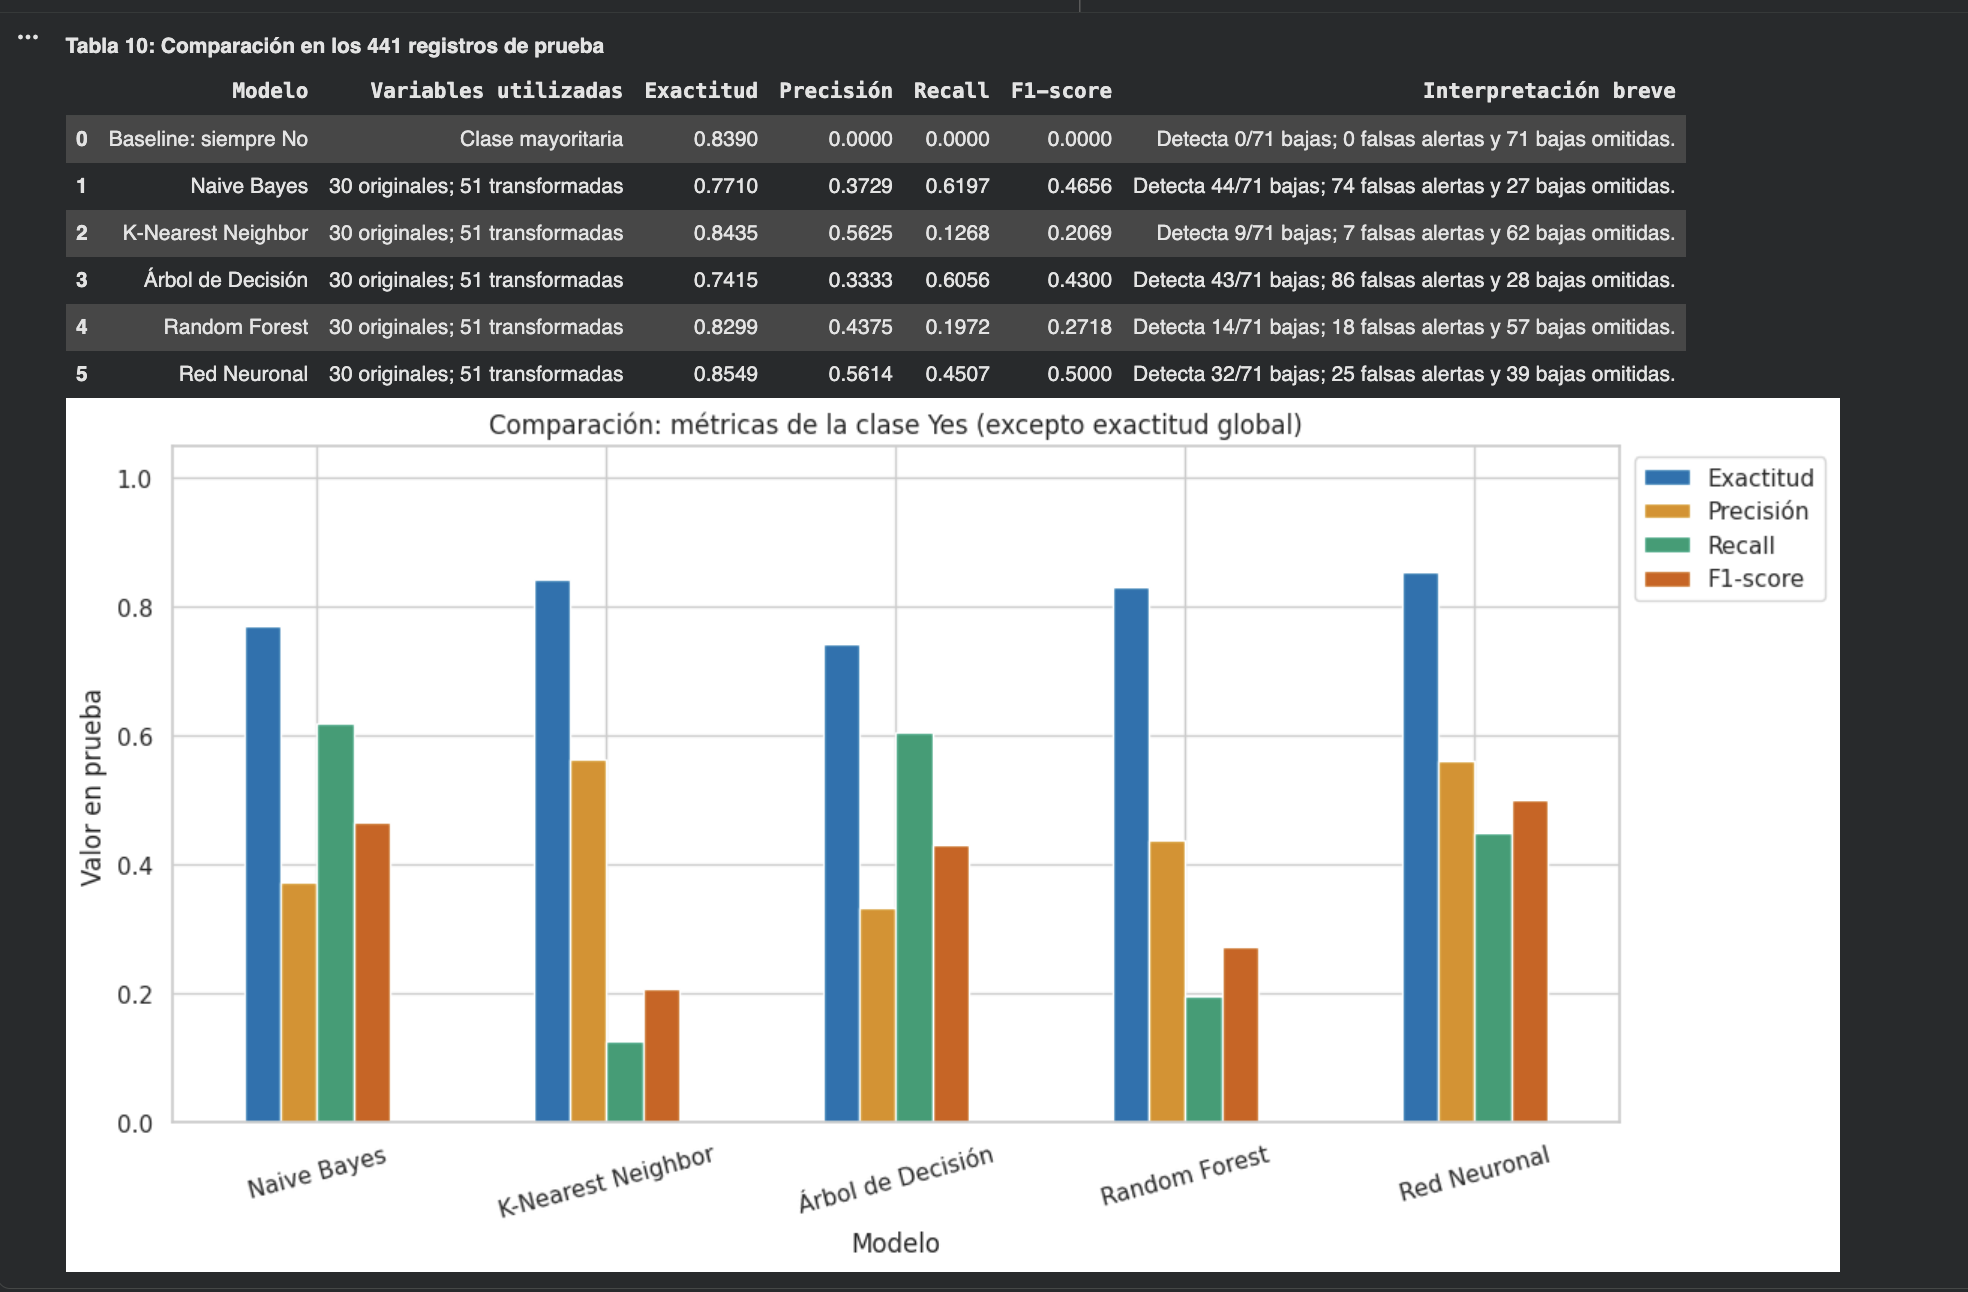
\includegraphics[width=\linewidth,height=0.4\textheight,keepaspectratio]{img/image13.png}
\caption{Tabla y grafica de comparacion de las metricas en prueba.}
\label{fig:comparacion-modelos}
\end{figure}

\subsection*{Análisis}
\addcontentsline{toc}{subsection}{Análisis}

La red neuronal obtuvo el mayor F1 en esta prueba y el mayor ROC-AUC. Detectó 32 de las 71 bajas, con 25 falsas alertas; todavía dejó 39 sin detectar. Naive Bayes reconoció más bajas, 44, pero generó 74 falsas alertas. El árbol tuvo un comportamiento similar, con 43 bajas detectadas y 86 falsas alertas.

En el caso de KNN, la exactitud fue alta (\textasciitilde{}0.84), pero solamente encontró nueve bajas. La referencia que siempre responde No obtiene casi 0.84 de exactitud y cero recall y F1 para bajas. Lo que esto nos quiere decir es que una exactitud cercana al 84\% puede obtenerse sin resolver el problema que nos interesa. Random Forest reconoció 14 bajas, por lo que su umbral de 0.5 resultó poco sensible a esta clase.

Se calculó ROC-AUC a partir de probabilidades y AP como resumen de la curva precision-recall. Estas curvas permiten revisar distintos umbrales. Las líneas de referencia corresponden a discriminación aleatoria en ROC y proporción de bajas en precision-recall.

\begin{figure}[H]
\centering
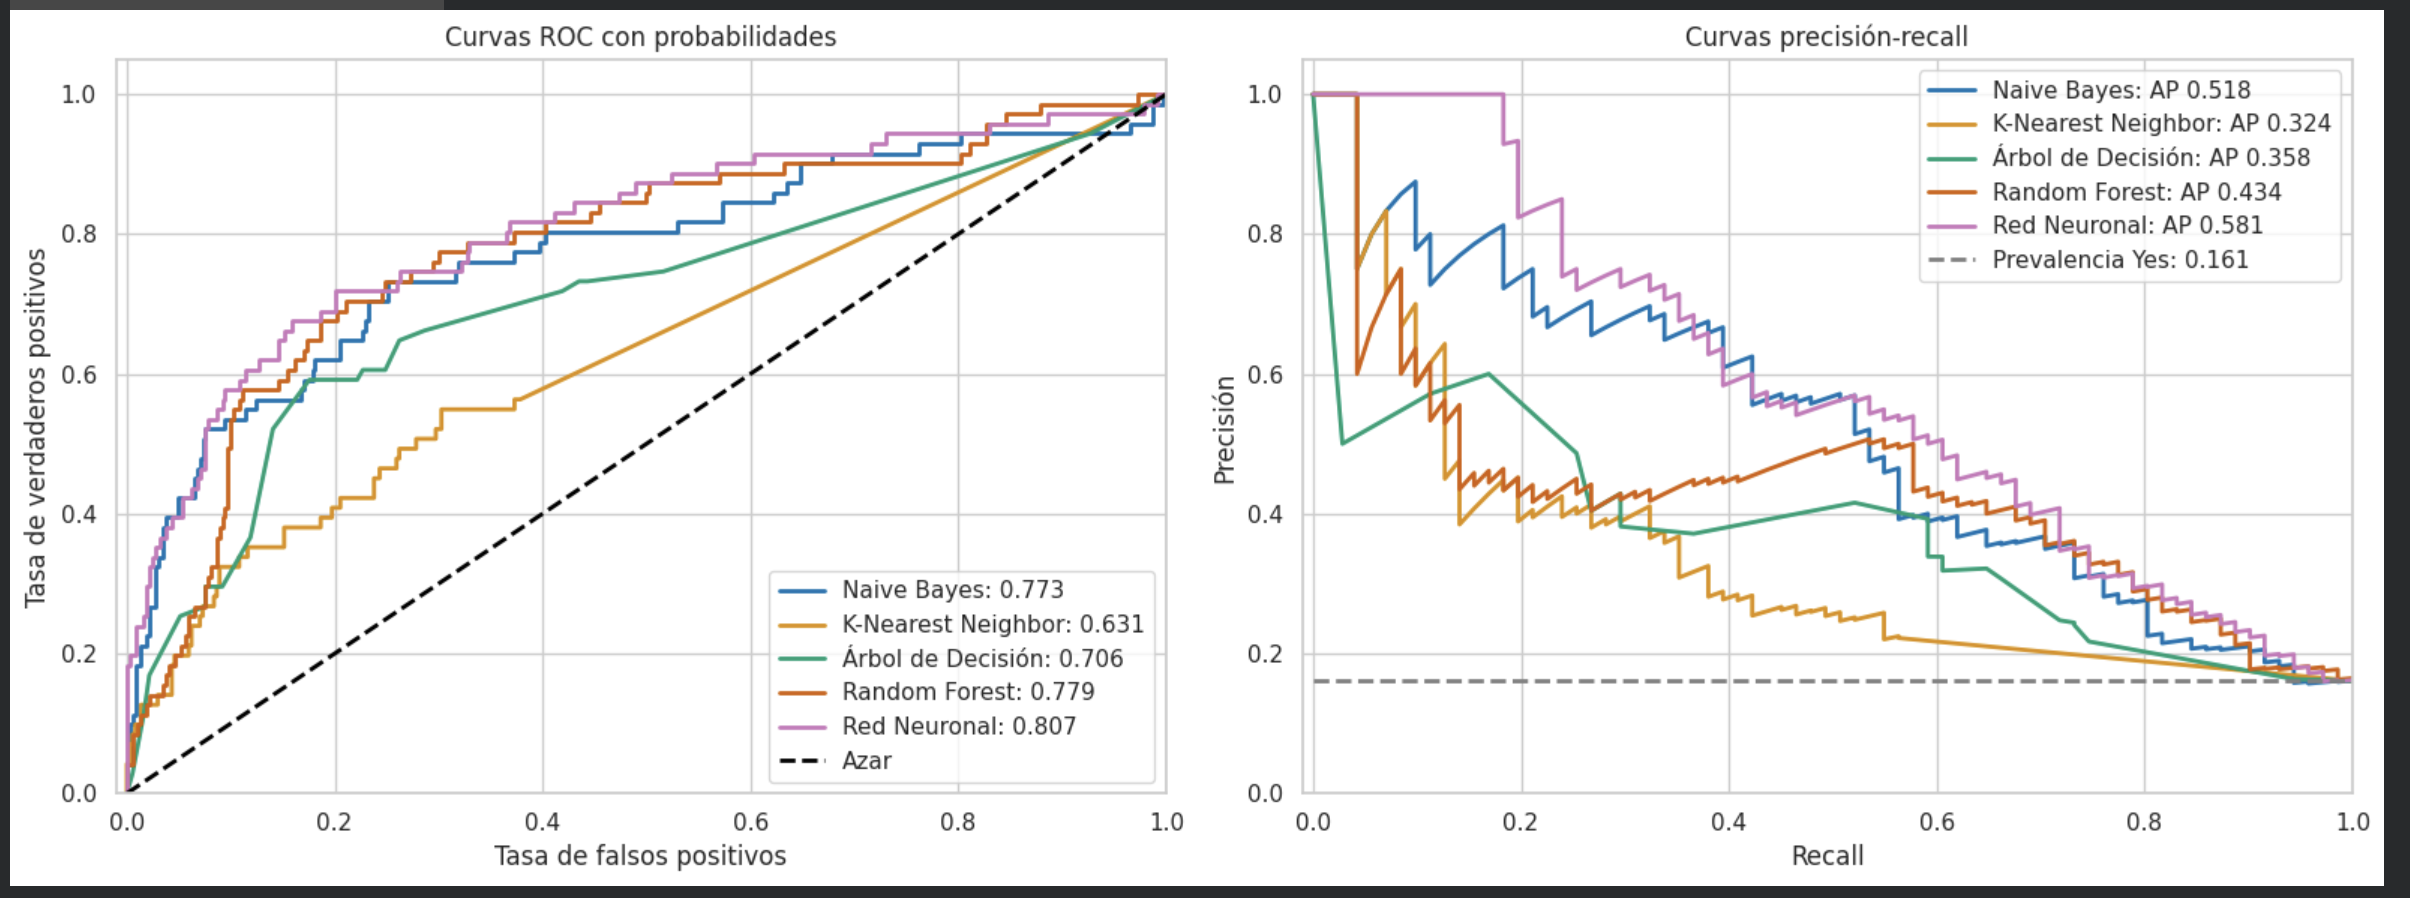
\includegraphics[width=\linewidth,height=0.78\textheight,keepaspectratio]{img/image14.png}
\caption{Comparacion de curvas ROC y precision-recall.}
\label{fig:roc-precision-recall}
\end{figure}

\section{Explicabilidad e interpretabilidad}


Para revisar qué variables tuvieron mayor influencia en los modelos se utilizó la importancia por permutación. Este método consiste en cambiar los valores de una columna en los datos de prueba y medir cuánto disminuye el ROC-AUC. Para cada modelo se hicieron cinco repeticiones. Si la caída es mayor, significa que el modelo dependió más de esa variable en esta prueba. Las barras de error muestran la variación entre las diferentes permutaciones y no representan un intervalo de confianza.

Se permutaron las columnas originales para mantener juntas las categorías que después se convierten en variables one-hot. Además, cuando dos variables están relacionadas, pueden repartirse la importancia entre ellas. Por otro lado, una importancia cercana a cero o negativa indica que la variable no tuvo una contribución constante en esta prueba. Estas gráficas permiten saber qué variables utiliza más el modelo, pero no demuestran que cambiar una condición laboral provoque una baja y tampoco se utilizan para volver a seleccionar las variables.

Las tablas muestran las 10 variables con mayor caída en ROC-AUC, mientras que las gráficas muestran solamente las 8 principales (Figura~\ref{fig:permutacion}). OverTime ocupa el primer lugar en los cinco modelos: su caída de ROC-AUC fue de 0.048 en Naive Bayes, 0.044 en KNN, 0.111 en el árbol, 0.081 en Random Forest y 0.070 en la red neuronal. Es la única variable que se mantiene como una de las principales en todos los modelos y coincide con lo observado en la Parte 2, donde el 30.5\% de los empleados con horas extra dejaron la empresa, frente al 10.4\% de los que no hacían horas extra.

Después de OverTime, el orden de importancia cambia dependiendo del modelo. En Naive Bayes destacan MaritalStatus y JobRole; en KNN, DailyRate y YearsAtCompany; en el árbol, JobLevel y StockOptionLevel; en Random Forest, EnvironmentSatisfaction y StockOptionLevel; y en la red neuronal, StockOptionLevel (nivel de opciones de acciones) y MonthlyIncome. Algunas barras de error son relativamente grandes en comparación con la caída, como ocurre con DailyRate en KNN o con Age y YearsAtCompany en el árbol. Por esto, considerando que solo hay 71 bajas en los datos de prueba, el orden de las variables secundarias debe tomarse como una referencia y no como una diferencia definitiva. Las caídas también son relativamente pequeñas porque, al cambiar una variable, las demás todavía conservan parte de la información que utiliza el modelo.

\begin{figure}[H]
\centering
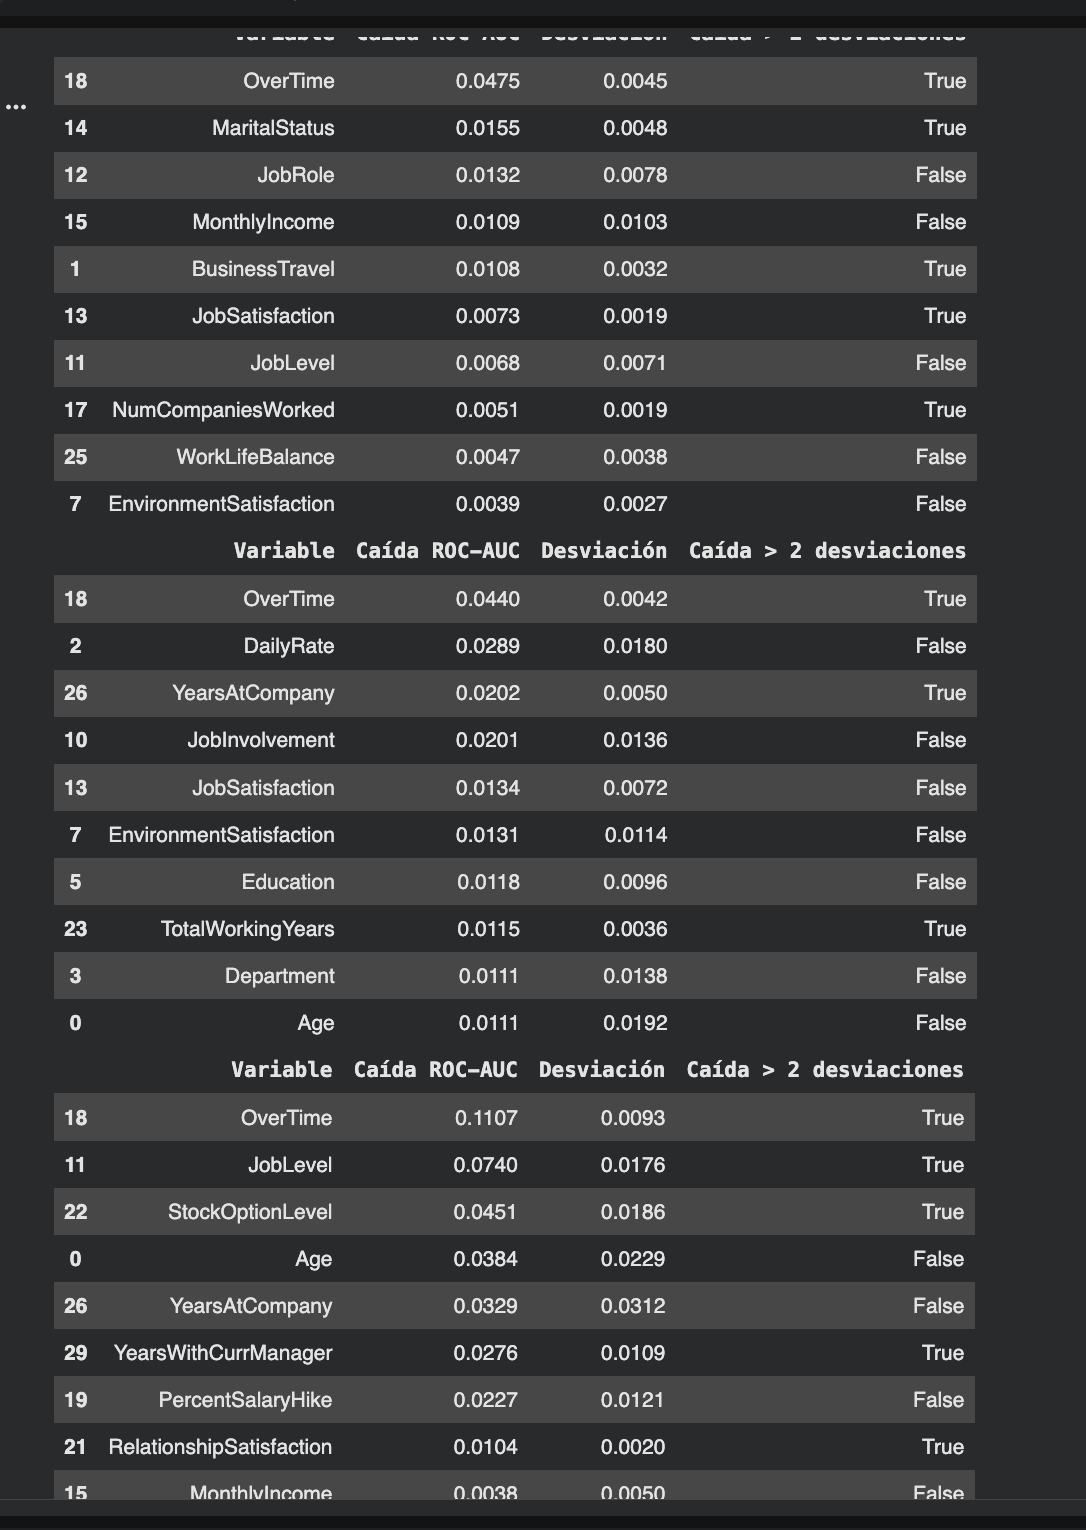
\includegraphics[width=\linewidth,height=0.78\textheight,keepaspectratio]{img/image15.png}
\caption{Salida de la importancia por permutacion de las variables.}
\label{fig:permutacion}
\end{figure}

\subsection*{6.2. Naive Bayes: probabilidades y explicacion de un caso}
\addcontentsline{toc}{subsection}{6.2. Naive Bayes: probabilidades y explicacion de un caso}
Para este análisis se obtuvieron las medias y varianzas que GaussianNB aprendió para cada clase. Se muestran diez variables que tienen diferencias grandes entre sus medias, junto con las probabilidades obtenidas para el primer registro de prueba. La tabla de contribuciones permite ver qué variables apoyan la predicción hacia Yes o hacia No: un valor positivo favorece Yes, mientras que uno negativo favorece No.

Las mayores diferencias entre las medias se encuentran principalmente en variables relacionadas con la experiencia y el nivel del empleado. Entre ellas están Age (\ensuremath{-}0.50), TotalWorkingYears (\ensuremath{-}0.50), YearsInCurrentRole (\ensuremath{-}0.47), YearsWithCurrManager (\ensuremath{-}0.46), JobLevel (\ensuremath{-}0.44), MonthlyIncome (\ensuremath{-}0.44) y YearsAtCompany (\ensuremath{-}0.44), en unidades estandarizadas. En todas ellas, los empleados que dejaron la empresa tienen valores más bajos. Como varias de estas variables están relacionadas entre sí, Naive Bayes las trata como si fueran independientes y suma su información para realizar la predicción.

El caso de prueba \#0, que corresponde a la posición original 397, es un error del modelo. La clase real es No, pero Naive Bayes asigna una probabilidad P(Yes) = 0.9039, partiendo de un prior de entrenamiento de 0.1613. Las variables que más apoyan la predicción Yes son OverTime (+0.5473 en cada una de sus dos columnas), Age (+0.5281), MaritalStatus\_Single (+0.4420), TotalWorkingYears (+0.3778) y MonthlyIncome (+0.3351). Por otro lado, JobSatisfaction aporta \ensuremath{-}0.3272, favoreciendo la clase No.

Además, OverTime\_No y OverTime\_Yes son columnas complementarias y aportan el mismo valor. Por esto, el modelo termina contando la información de OverTime dos veces, con una contribución aproximada de 1.09 en log-odds. Esto muestra una de las limitaciones de Naive Bayes: la independencia entre las variables es solo una aproximación.

Finalmente, una probabilidad de 0.90 en un caso que realmente pertenece a No muestra que el modelo puede ser demasiado confiado en algunas predicciones. Naive Bayes detectó 44 de las 71 bajas, obteniendo un recall de 0.6197, pero también generó 74 falsas alertas y tuvo una precisión de 0.3729. Por esto, sus probabilidades deberían revisarse mediante una calibración antes de considerar su uso fuera de este ejercicio.

\begin{figure}[H]
\centering
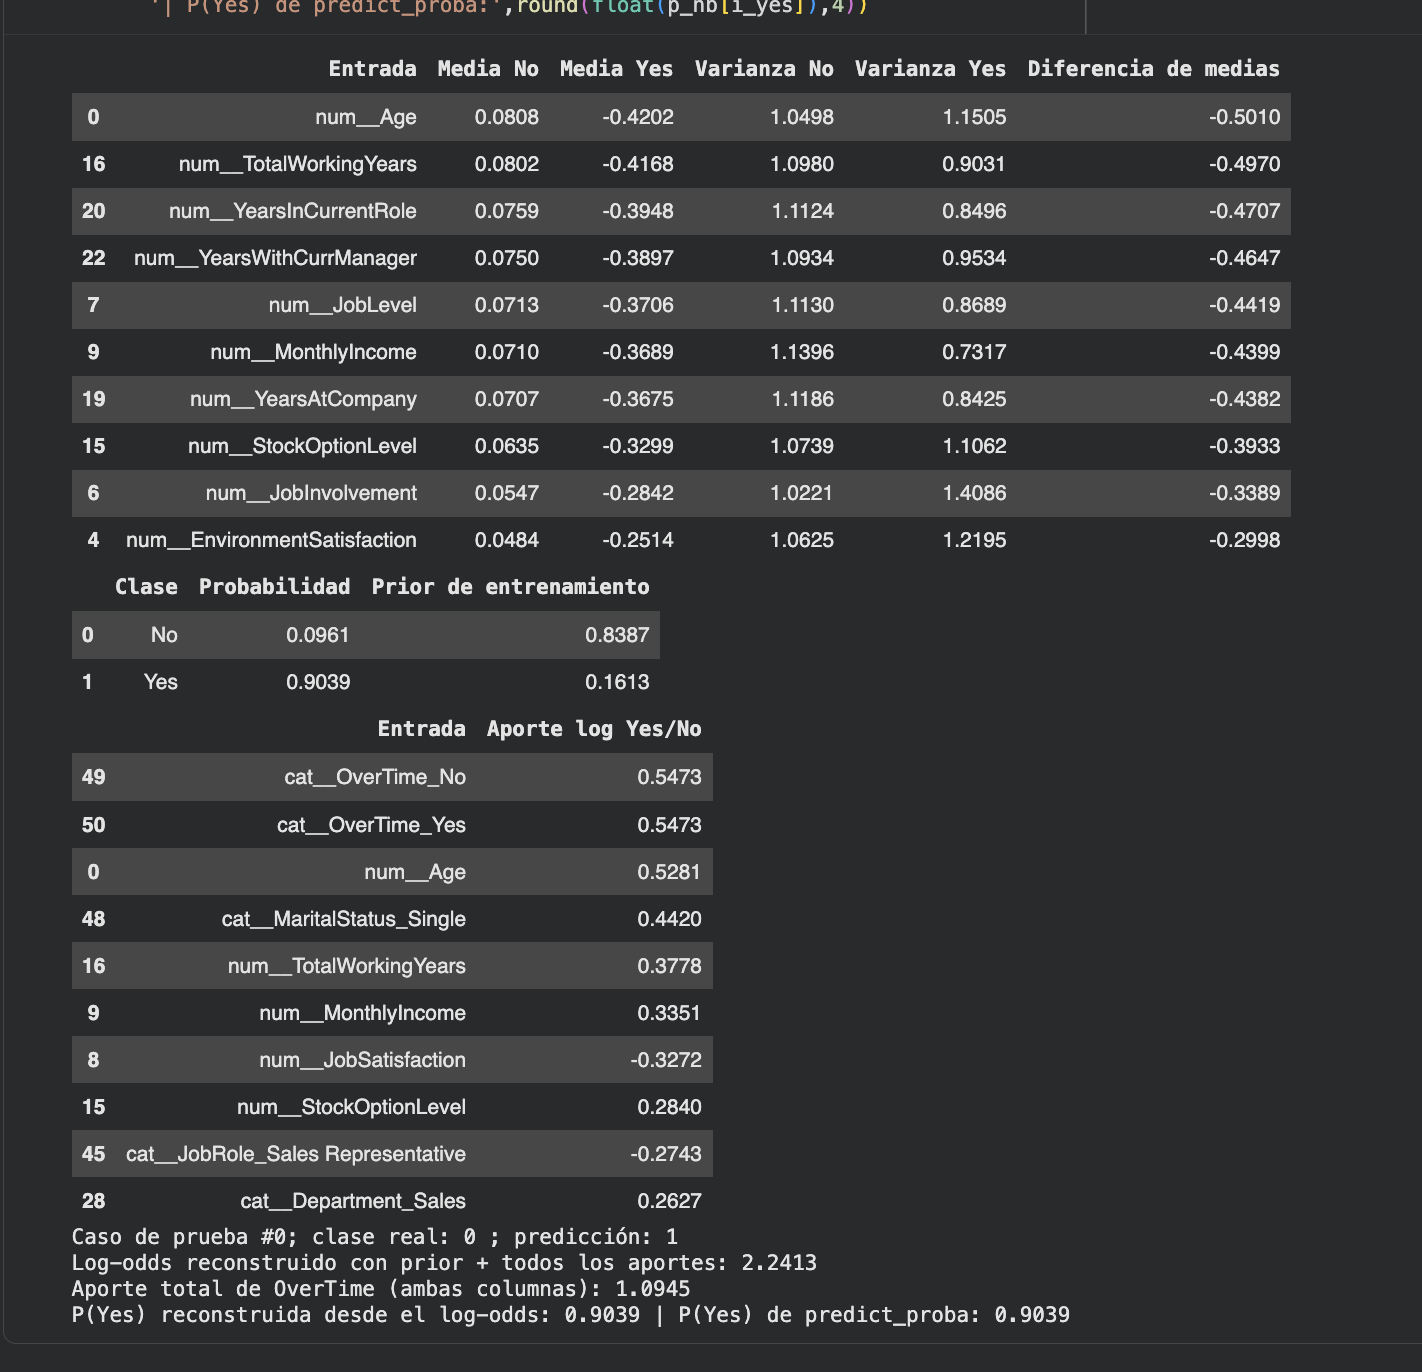
\includegraphics[width=\linewidth,height=0.5\textheight,keepaspectratio]{img/image16.png}
\caption{Parametros, probabilidades y contribuciones de Naive Bayes para el caso de prueba 0.}
\label{fig:naive-bayes}
\end{figure}

\subsection*{6.3. KNN: vecinos y votacion}
\addcontentsline{toc}{subsection}{6.3. KNN: vecinos y votacion}
Se revisaron los vecinos del primer registro de prueba, utilizando únicamente registros del conjunto de entrenamiento. La tabla muestra la distancia después de aplicar el escalado y la transformación one-hot, la clase real de cada vecino y su peso en la votación. También se comparan algunas características como edad, ingreso, horas extra y antigüedad para entender mejor qué registros considera cercanos el modelo.

El registro \#0 tiene 25 años, un ingreso de 4,487, hace horas extra y lleva 5 años en la empresa. Sus cinco vecinos pertenecen a la clase No, por lo que KNN obtiene P(Yes) = 0 y acierta la predicción. Los vecinos tienen entre 27 y 37 años, entre 4 y 6 años en la empresa e ingresos de 4,478 a 8,103. Además, cuatro de los cinco hacen horas extra. Esto significa que los registros se parecen considerando el conjunto de variables, y no por una sola característica. La distancia se calcula utilizando las 51 entradas del modelo, no solamente las cuatro variables que se muestran en la tabla.

Las distancias están entre 3.64 y 4.05, mientras que los pesos de votación van de 0.189 a 0.210, por lo que son bastante parecidos. Con 51 variables, la diferencia entre el vecino más cercano y el quinto es pequeña. Una distancia menor solamente indica que los registros son parecidos después de aplicar las transformaciones del modelo, pero no significa que tengan la misma causa de rotación.

Esto ayuda a explicar el desempeño de KNN en la Parte 5. El modelo detectó solamente 9 de las 71 bajas, obteniendo un recall de 0.1268. Para predecir Yes, la mayoría de los vecinos debe pertenecer a esa clase, algo que ocurre pocas veces porque las bajas representan solo el 16\% de los empleados. Por esto, aunque obtuvo un F1 de 1.0000 en entrenamiento, en prueba bajó a 0.2069. Finalmente, EmployeeNumber no se utilizó como predictor porque solamente funciona como identificador del empleado.

\begin{figure}[H]
\centering
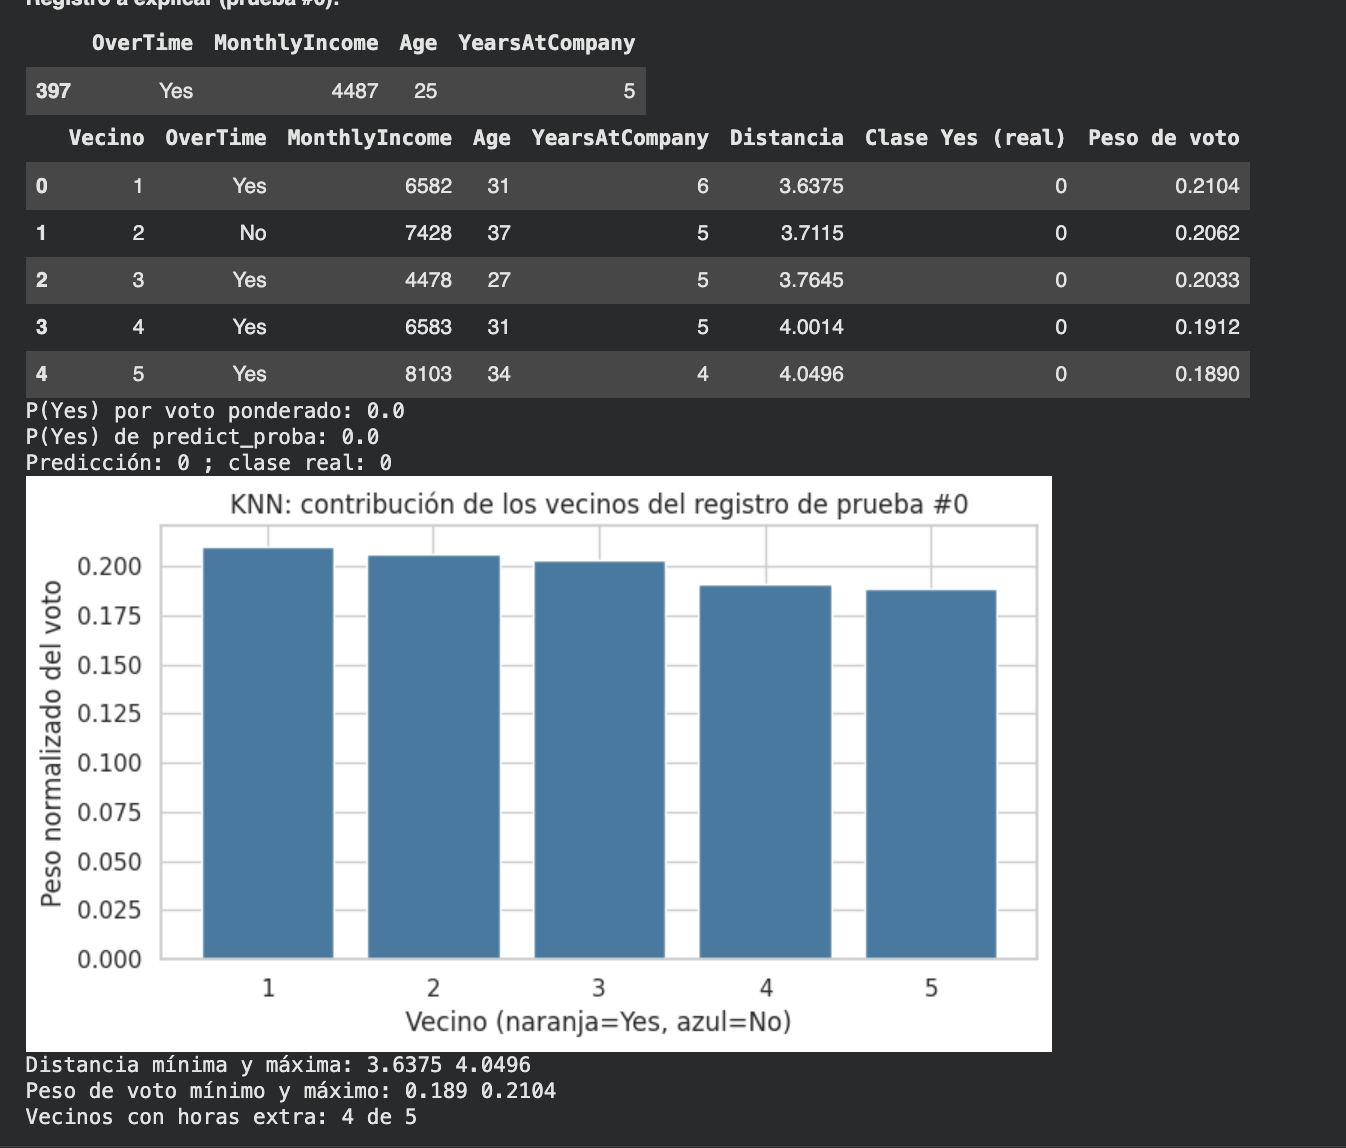
\includegraphics[width=\linewidth,height=0.35\textheight,keepaspectratio]{img/image17.png}
\caption{Vecinos y pesos de votacion de KNN para el caso de prueba 0.}
\label{fig:vecinos-knn}
\end{figure}

\subsection*{6.4. Arbol de decision: reglas y recorrido}
\addcontentsline{toc}{subsection}{6.4. Arbol de decision: reglas y recorrido}
Se dibujó el árbol mostrando hasta la profundidad 3, aunque su profundidad real es 5. Las reglas completas se guardaron en 15\_reglas\_arbol.txt y también se muestra el recorrido que sigue el primer caso de prueba. samples indica cuántos registros llegan a cada nodo, mientras que value considera los pesos de las clases debido a class\_weight='balanced'. Por esto, los valores de value no coinciden directamente con samples. En las variables numéricas, los cortes mantienen sus unidades originales, mientras que en las variables one-hot un corte de 0.5 sirve para separar entre la categoría ausente y presente.

La raíz del árbol divide usando YearsAtCompany <= 2.5. Los empleados con 2.5 años o menos en la empresa (238 de los 1,029 registros de entrenamiento) pasan a una rama donde predomina Yes. Los que tienen más antigüedad pasan a una división por OverTime: quienes hacen horas extra (226 registros) llegan a un nodo clasificado como Yes, mientras que quienes no hacen horas extra (565) llegan a uno clasificado como No. De esta forma, el árbol resume dos perfiles que tienen mayor riesgo de baja: tener poca antigüedad, o tener más antigüedad y hacer horas extra.

Aunque la raíz utiliza YearsAtCompany, la importancia por permutación de la sección 6.1 coloca a OverTime en primer lugar. Esto no es una contradicción, ya que las dos medidas analizan cosas diferentes. El primer corte indica qué variable permite separar mejor las clases en ese punto del entrenamiento, mientras que la permutación mide cuánto disminuye el desempeño en los datos de prueba cuando se altera una variable.

Para el caso \#0, el recorrido comienza con YearsAtCompany = 5, por lo que cumple > 2.5. Después, OverTime\_No = 0 cumple \ensuremath{\leq} 0.5, lo que indica que el empleado sí hace horas extra. El recorrido continúa con JobLevel = 2 (> 1.5), StockOptionLevel = 0 (\ensuremath{\leq} 0.5) y YearsWithCurrManager = 3 (> 2.5). Finalmente, el árbol llega a una hoja que predice Yes, aunque la clase real es No. Por lo tanto, comete el mismo falso positivo que Naive Bayes. Este recorrido permite ver las condiciones que llevaron al modelo a tomar esa decisión.

En conjunto, el árbol detectó 43 de las 71 bajas y generó 86 falsas alertas, obteniendo una precisión de 0.3333.

\begin{table}[H]
\centering
\footnotesize
\setlength{\tabcolsep}{5pt}
\caption{Recorrido real del caso de prueba 0 dentro del arbol completo.}
\label{tab:ruta}
\begin{tabular}{lrrrr}
\toprule
Nodo & Variable & Valor del caso & Umbral & Rama \\
\midrule
0 & YearsAtCompany & 5.0 & 2.5 & $>$ \\
24 & OverTime\_No & 0.0 & 0.5 & $\leq$ \\
25 & JobLevel & 2.0 & 1.5 & $>$ \\
31 & StockOptionLevel & 0.0 & 0.5 & $\leq$ \\
32 & YearsWithCurrManager & 3.0 & 2.5 & $>$ \\
\bottomrule
\end{tabular}
\end{table}

\begin{figure}[H]
\centering
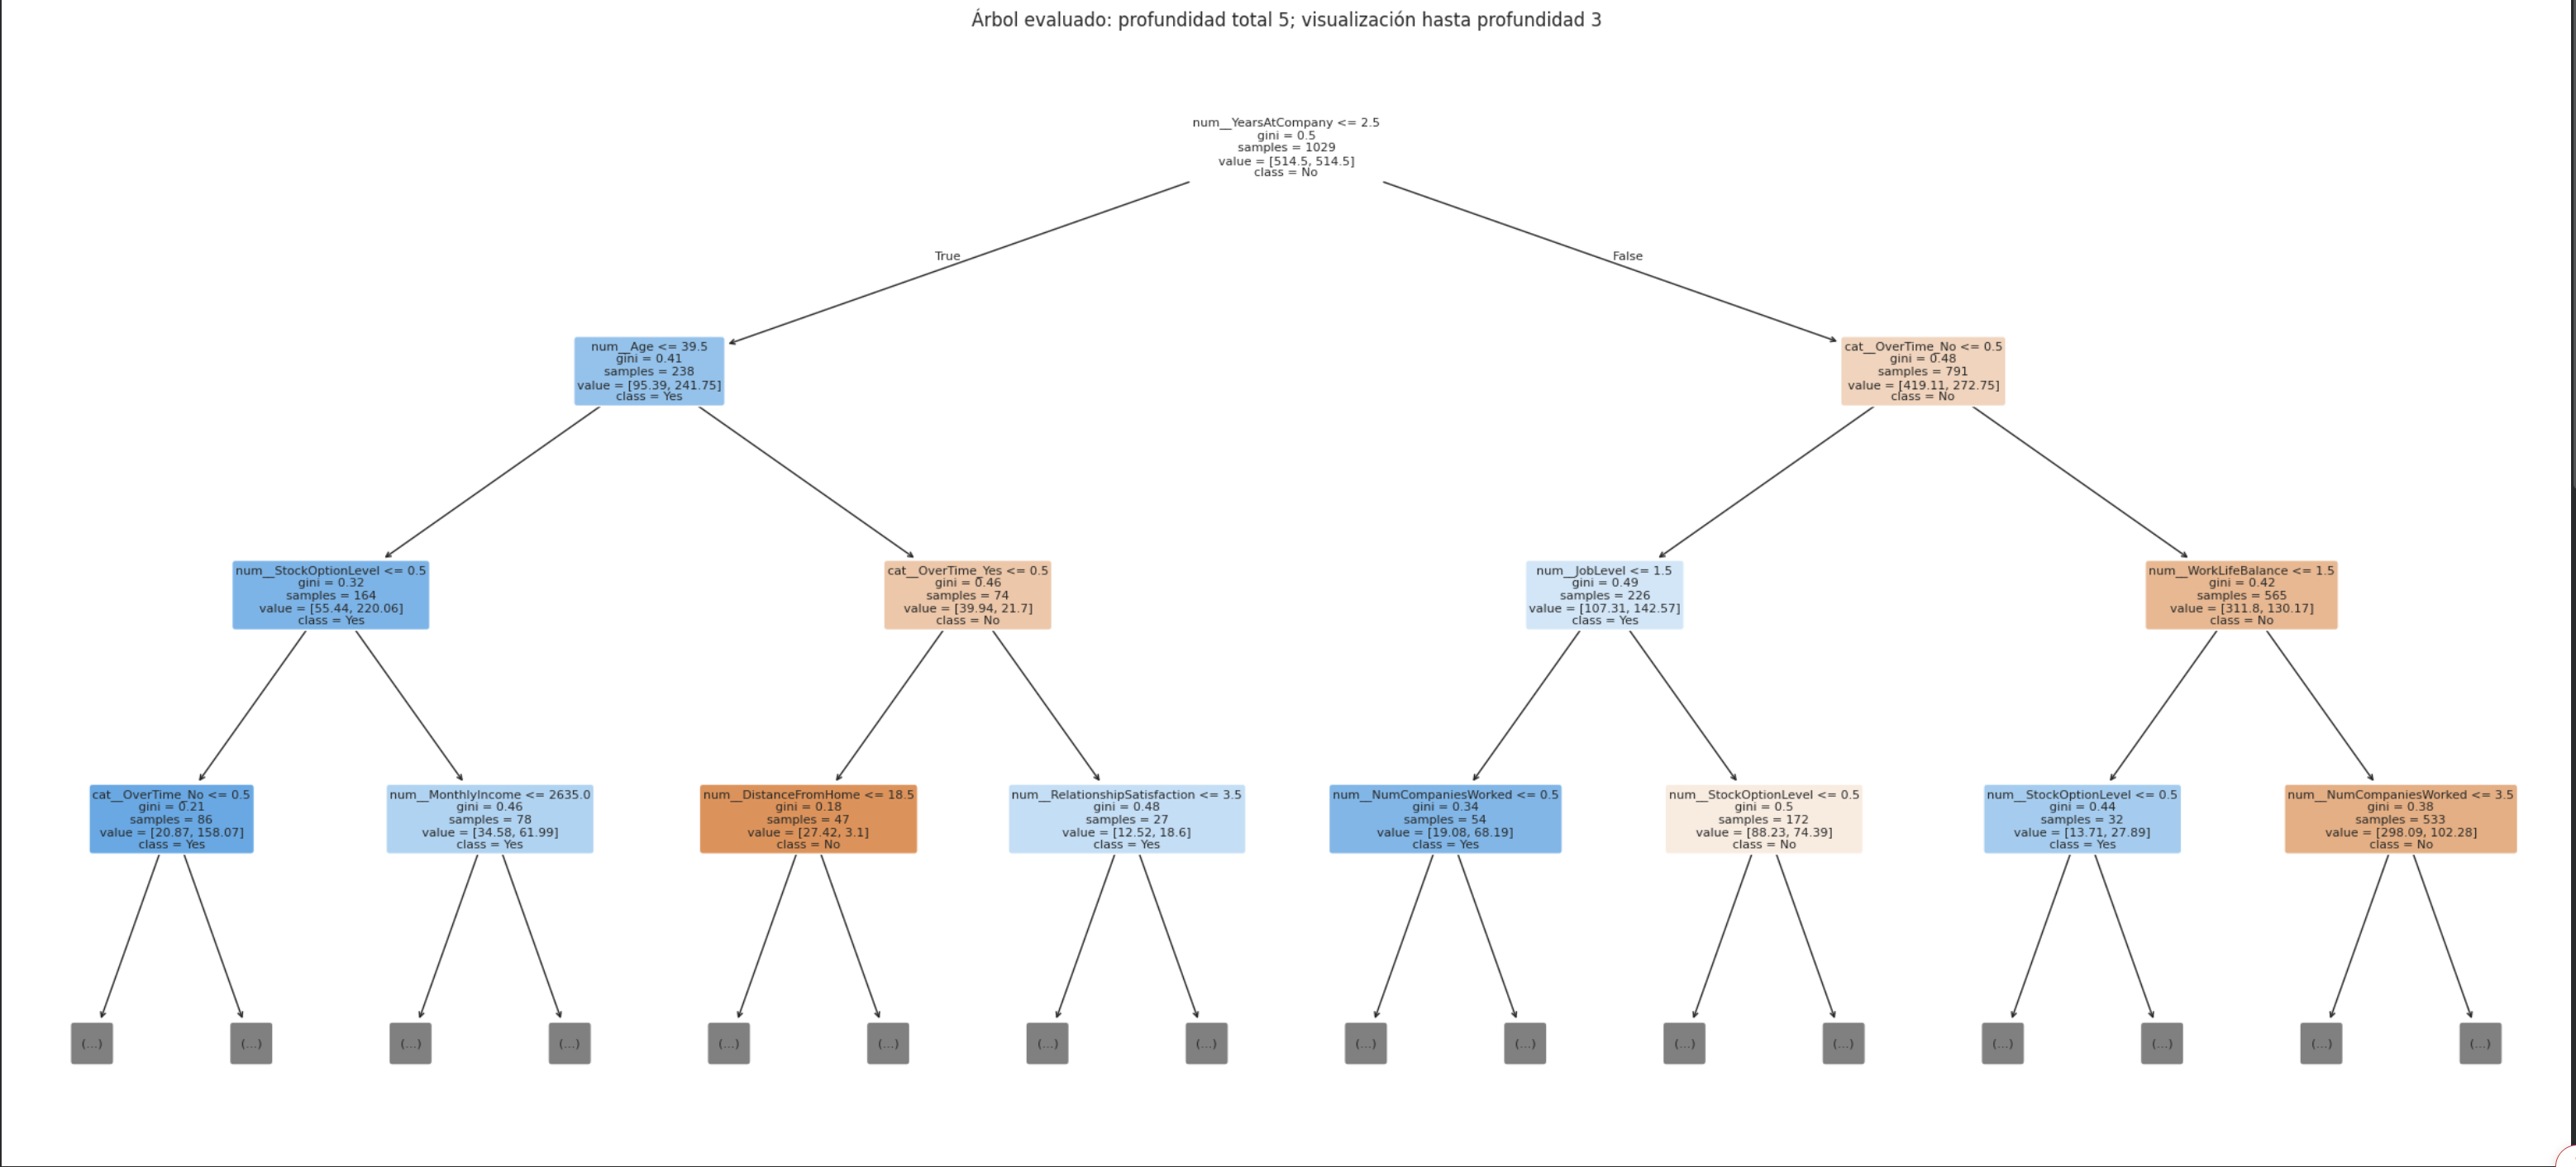
\includegraphics[width=\linewidth,height=0.78\textheight,keepaspectratio]{img/image18.png}
\caption{Arbol de decision visualizado hasta la profundidad 3.}
\label{fig:arbol-decision}
\end{figure}

\newpage
\subsection*{6.5. Random Forest: importancia de las variables}
\addcontentsline{toc}{subsection}{6.5. Random Forest: importancia de las variables}
Random Forest combina las predicciones de 200 árboles. Para analizar qué variables utiliza más, se obtuvo la importancia por reducción de impureza y se sumaron las categorías de one-hot para volver a las variables originales. Después, estos resultados se compararon con la importancia por permutación .

Las dos medidas muestran resultados diferentes. Por reducción de impureza destacan MonthlyIncome (0.0838), OverTime (0.0720), Age (0.0655) y TotalWorkingYears (0.0534). También aparecen entre las primeras DailyRate (0.0471), MonthlyRate (0.0398) y HourlyRate (0.0392). En cambio, por permutación, OverTime es claramente la primera (0.0807), seguida de EnvironmentSatisfaction, StockOptionLevel, JobSatisfaction y JobInvolvement. MonthlyIncome baja al sexto lugar y tiene una barra de error grande. Age y DailyRate quedan entre las últimas posiciones, con caídas muy pequeñas, mientras que MonthlyRate y HourlyRate ya no aparecen entre las diez principales.

Esta diferencia muestra que la reducción de impureza puede dar más importancia a las variables continuas que tienen muchos posibles puntos de corte. Además, esta medida se calcula con los datos de entrenamiento, donde el bosque está sobreajustado, ya que obtuvo un F1 de 0.9790 en entrenamiento frente a 0.2718 en prueba. Por esto, para este análisis se considera más confiable la importancia por permutación. Aun así, hay una coincidencia importante: OverTime es la única variable que se mantiene entre las principales en ambas medidas. También hay que recordar que una importancia alta no indica por sí sola si una variable aumenta o disminuye la probabilidad de baja.

En esta prueba, Random Forest obtuvo un ROC-AUC de 0.7777, pero con un umbral de 0.5 solamente detectó 14 de las 71 bajas, obteniendo un recall de 0.1972. Para el caso \#0, el modelo asigna P(Yes) = 0.3904 y predice permanencia (No), por lo que acierta. Sin embargo, su baja sensibilidad muestra que sería interesante analizar otros umbrales en una evaluación posterior, utilizando validación y manteniendo los datos de prueba separados.

\begin{figure}[H]
\centering
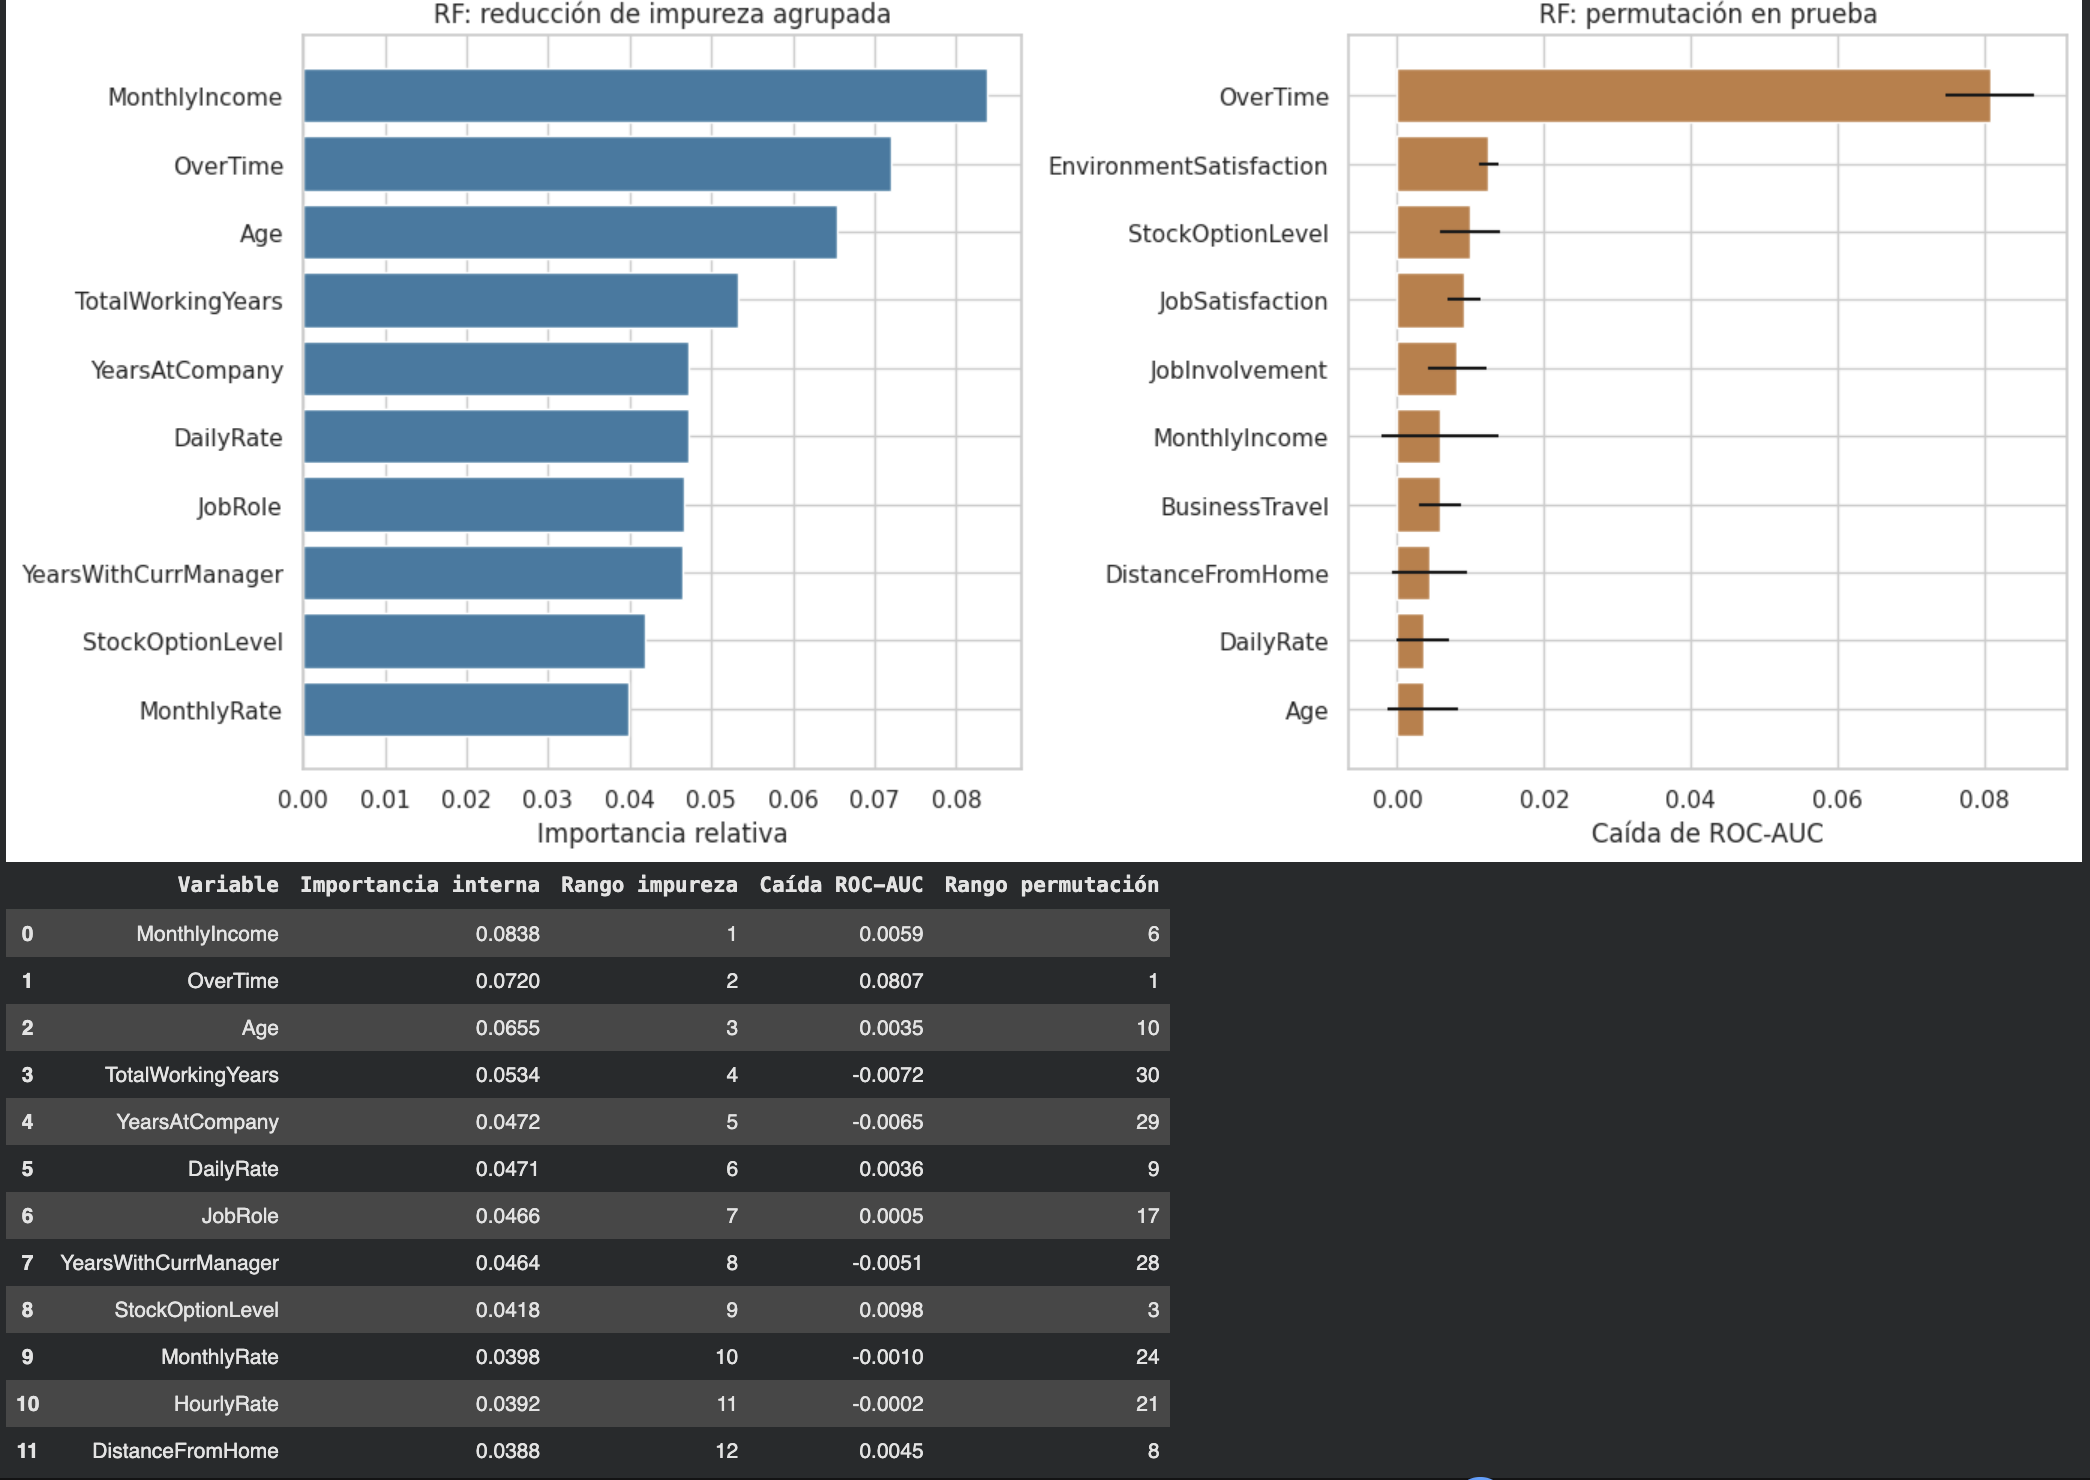
\includegraphics[width=\linewidth,height=0.4\textheight,keepaspectratio]{img/image19.png}
\caption{Importancia por reduccion de impureza y por permutacion en Random Forest.}
\label{fig:importancia-random-forest}
\end{figure}

\subsection*{6.6. Red neuronal: capas, pesos y entrenamiento}
\addcontentsline{toc}{subsection}{6.6. Red neuronal: capas, pesos y entrenamiento}

Se obtuvieron los tamaños de las capas, los pesos y los sesgos de la red entrenada. La arquitectura es 51 \ensuremath{\rightarrow} 20 \ensuremath{\rightarrow} 10 \ensuremath{\rightarrow} 1, con dos capas ocultas que utilizan ReLU y una neurona de salida logística que calcula $P(\text{Yes})$. La red tiene 1,230 pesos y 31 sesgos, además de regularización L2 ($\alpha = 1$) y el optimizador Adam. El diagrama muestra todos los nodos y conexiones, usando azul para los pesos positivos, naranja para los negativos y un mayor grosor para los pesos de mayor magnitud. Sin embargo, con 1,230 conexiones es difícil de leer, por lo que resulta más útil observar el mapa de calor de los pesos de la primera capa y la curva de pérdida.

El entrenamiento terminó en 379 iteraciones, con una pérdida final de 0.1712, sin alcanzar max\_iter. Esta pérdida incluye la regularización y corresponde a los datos de entrenamiento, por lo que una disminución de la pérdida no significa necesariamente que la red tendrá el mismo desempeño con datos nuevos. Esto se observa en el F1, que fue de 0.9304 en entrenamiento y bajó a 0.5000 en prueba. Por lo tanto, existe sobreajuste, aunque la red neuronal fue el modelo con mejor desempeño en los datos de prueba. En el mapa de calor se observan pesos positivos y negativos distribuidos entre las 20 neuronas de la primera capa. No hay una sola entrada que domine, y un peso aislado tampoco permite determinar la importancia de una variable, ya que la predicción depende de las capas siguientes.

Para analizar la influencia de las variables se utilizó la importancia por permutación de la Figura~\ref{fig:permutacion}. Las variables que más destacan en la red son OverTime, con una caída de 0.0700, StockOptionLevel, MonthlyIncome y JobSatisfaction. De estas, OverTime es la más importante y también fue la variable que se mantuvo como principal en los demás modelos.

La tabla final compara los cinco modelos utilizando el mismo registro \#0, cuya clase real es No. Naive Bayes (P(Yes) = 0.9039) y el árbol de decisión generan una falsa alerta. En cambio, KNN (P(Yes) = 0), Random Forest (P(Yes) = 0.3904) y la red neuronal (P(Yes) = 0.1980) predicen permanencia y aciertan. Esto muestra que modelos con diferente desempeño general pueden dar respuestas distintas para un mismo registro. También se puede observar que una probabilidad alta, como la de Naive Bayes, no garantiza que la predicción sea correcta. Sin embargo, un solo caso no permite comparar cuál modelo es mejor; solamente sirve para mostrar cómo se comporta cada uno ante el mismo empleado.

\begin{table}[H]
\centering
\small
\setlength{\tabcolsep}{5pt}
\caption{Capas y parametros extraidos de la red entrenada.}
\label{tab:mlp}
\begin{tabular}{lrrrrr}
\toprule
Conexion & Entradas & Salidas & Pesos & Sesgos & Media $|w|$ \\
\midrule
51 $\rightarrow$ 20 & 51 & 20 & 1020 & 20 & 0.0712 \\
20 $\rightarrow$ 10 & 20 & 10 & 200 & 10 & 0.1823 \\
10 $\rightarrow$ 1 & 10 & 1 & 10 & 1 & 0.7823 \\
\bottomrule
\end{tabular}
\end{table}

\begin{figure}[H]
\centering
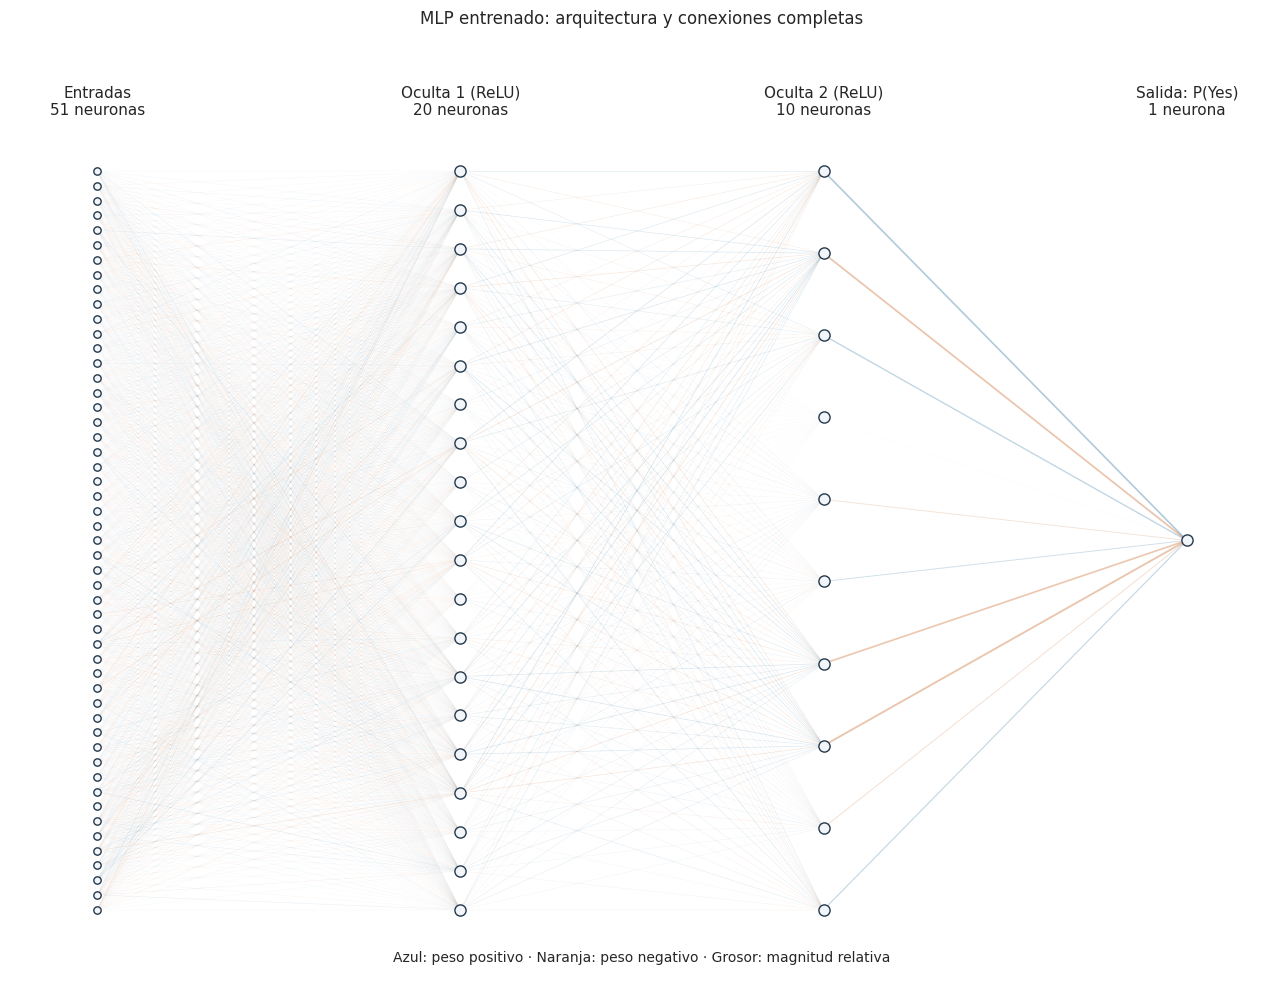
\includegraphics[width=\linewidth,height=0.78\textheight,keepaspectratio]{img/image20.png}
\caption{Arquitectura y conexiones de la red neuronal entrenada.}
\label{fig:arquitectura-red}
\end{figure}

\begin{figure}[H]
\centering
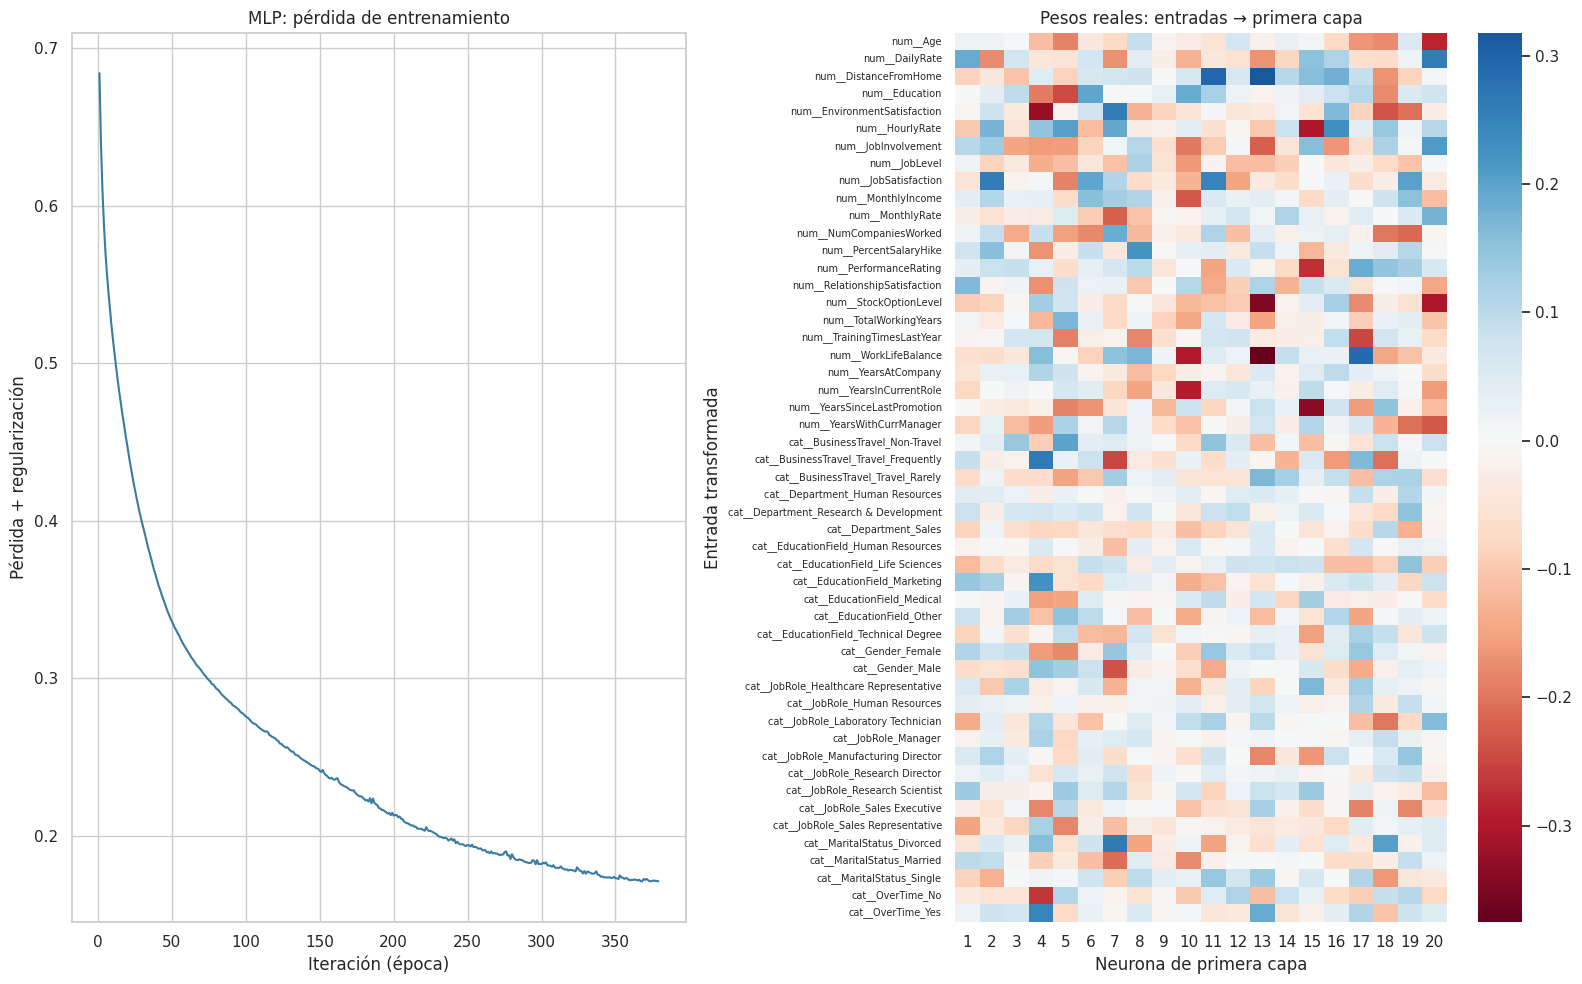
\includegraphics[width=\linewidth,height=0.78\textheight,keepaspectratio]{img/image21.png}
\caption{Curva de perdida y mapa de calor de los pesos de la primera capa.}
\label{fig:entrenamiento-red}
\end{figure}

\begin{figure}[H]
\centering
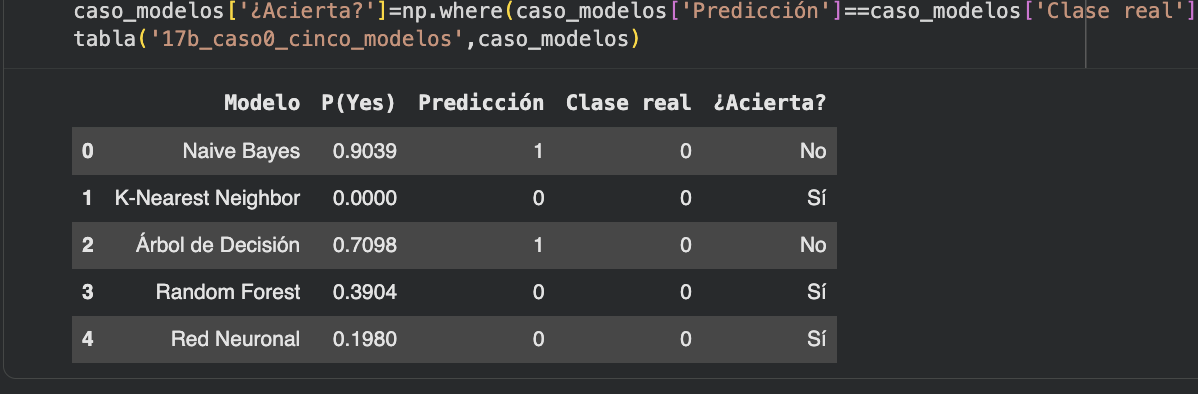
\includegraphics[width=\linewidth,height=0.78\textheight,keepaspectratio]{img/image22.png}
\caption{Predicciones de los cinco modelos para el mismo caso de prueba.}
\label{fig:comparacion-caso}
\end{figure}

\subsection*{6.7. Revision de resultados por genero}
\addcontentsline{toc}{subsection}{6.7. Revision de resultados por genero}
Por último, se revisó el modelo seleccionado mediante validación cruzada, que en este caso fue la red neuronal, separando los resultados por género. Para cada grupo se muestra su tamaño, las bajas reales, las bajas detectadas, las falsas alertas, la precisión, el recall y el F1. Cuando alguna métrica no puede calcularse, se conserva como NaN. Gender sí forma parte de las variables de entrada del modelo, por lo que esta revisión analiza directamente un modelo que utiliza esta información.

La tasa de bajas es parecida entre ambos grupos: 15.4\% en mujeres y 16.5\% en hombres. En el grupo Female se detectaron 13 de 26 bajas, con un recall de 0.5000, mientras que en Male se detectaron 19 de 45, con un recall de 0.4222. La tasa de falsos positivos fue de 0.063 para mujeres y 0.071 para hombres. Aunque existe una diferencia en el recall, esta representa solamente entre dos y cuatro empleados. Por el tamaño de los grupos, estos resultados no son suficientes para concluir que el modelo discrimine por género, pero tampoco permiten asegurar que esté libre de posibles sesgos.

Para hacer una revisión más completa sería necesario analizar otras variables sensibles o que puedan estar relacionadas con ellas, como Age y MaritalStatus, esta última entre las variables más importantes de Naive Bayes. También sería útil comparar el desempeño del modelo con Gender y sin Gender. Quitar directamente una variable sensible no significa que desaparezca su posible influencia, ya que otras variables pueden estar relacionadas con ella. Finalmente, también se debe revisar que las variables utilizadas por el modelo sean datos que realmente estén disponibles antes de que ocurra una baja.

\begin{figure}[H]
\centering
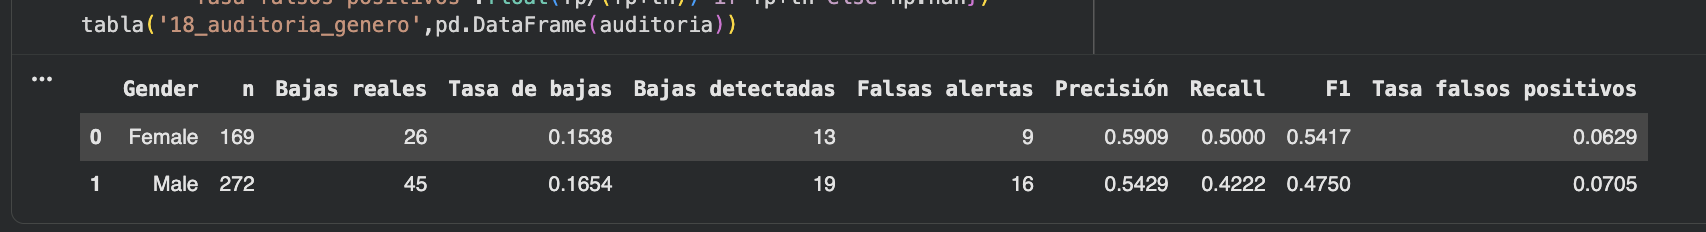
\includegraphics[width=\linewidth,height=0.78\textheight,keepaspectratio]{img/image23.png}
\caption{Salida de la revision de resultados por genero.}
\label{fig:revision-genero}
\end{figure}

\section{Preguntas}


\subsection*{1. ¿Cual fue la variable objetivo y por que es relevante para el negocio?}

La variable objetivo utilizada fue Attrition (Yes = 1, No = 0), la cual indica si un empleado dejó la empresa o si continúa trabajando en ella. Esta variable es importante porque la salida de un empleado puede generar diferentes gastos para la empresa, como la contratación y capacitación de una nueva persona. Además, también se puede perder experiencia y conocimiento que el trabajador adquirió durante el tiempo que estuvo en la organización. Por esta razón, contar con un modelo que permita identificar a los empleados con mayor riesgo de dejar la empresa podría ayudar a tomar medidas para intentar reducir estas bajas y priorizar acciones de retención.

El conjunto de datos contiene 1,470 empleados, de los cuales 237 dejaron la empresa, lo que representa aproximadamente el 16.1\%. Esto significa que la mayoría de los empleados permanecieron en su puesto, por lo que existe una diferencia importante entre las dos clases. Debido a esto, no es suficiente evaluar el modelo únicamente con la exactitud (accuracy). Por ejemplo, un modelo que siempre prediga No tendría una exactitud del 83.9\%, pero no sería capaz de detectar ninguna de las bajas reales. Por lo tanto, también es necesario utilizar otras métricas que permitan conocer qué tan bien el modelo identifica a los empleados que dejaron la empresa.

Además, en una aplicación real sería necesario definir desde qué momento se toman los datos y durante qué periodo se quiere predecir la posible baja. Esto permitiría saber si las variables utilizadas por el modelo realmente estarían disponibles antes de que el empleado deje la empresa.

\subsection*{2. ¿Que variables se consideraron mas importantes despues del EDA?}

Durante el EDA (análisis exploratorio de datos) se encontraron algunas diferencias importantes entre los empleados que dejaron la empresa y los que permanecieron. La variable que más destacó fue OverTime, ya que el 30.5\% de los empleados que hacían horas extra dejaron la empresa, mientras que entre los que no hacían horas extra la tasa fue de 10.4\%. También destacó JobRole, donde los Sales Representative tuvieron un 39.8\% de bajas, aunque este resultado debe tomarse con cuidado porque solo había 83 empleados en ese puesto. En Department, el área de Sales presentó un 20.6\% de bajas, frente al 13.8\% de Research \& Development.

También se compararon MonthlyIncome y YearsAtCompany. Los empleados que dejaron la empresa tenían un ingreso mensual promedio de 4,787 y 5.13 años en la compañía, mientras que los que permanecieron tenían un ingreso promedio de 6,833 y 7.37 años. Estas diferencias permiten observar algunos patrones en los datos, pero no significan que una variable sea necesariamente la causa de que un empleado deje la empresa.

Después del EDA, al entrenar los modelos se utilizó la importancia por permutación para analizar qué variables eran más utilizadas por cada modelo. En la red neuronal destacaron OverTime, StockOptionLevel, MonthlyIncome, JobSatisfaction y TotalWorkingYears. Sin embargo, la importancia de las demás variables cambió dependiendo del modelo. OverTime fue la única variable que se mantuvo como la más importante en los cinco modelos, por lo que fue el resultado más constante. Finalmente, se eliminaron EmployeeNumber porque solo funciona como identificador, y EmployeeCount, StandardHours y Over18 porque tenían el mismo valor para todos los empleados.

Es importante diferenciar ambos análisis: el EDA permite observar diferencias y patrones directamente en los datos, mientras que la importancia por permutación muestra cuánto cambia el desempeño del modelo cuando se modifica una variable. Ninguno de los dos análisis demuestra por sí solo que una variable sea la causa de la rotación de empleados.

\subsection*{3. ¿Que modelo obtuvo el mejor desempeño y con que metrica se justifica?}

El mejor desempeño lo obtuvo la Red Neuronal, principalmente por su valor de F1 = 0.5000 para la clase Yes. Esta métrica es importante porque toma en cuenta tanto las bajas que el modelo logra detectar como las falsas alertas, por lo que resulta adecuada debido al desbalance entre las clases. Además, obtuvo una precisión de 0.5614, un recall de 0.4507, una exactitud de 0.8549, un ROC-AUC de 0.8075 y un AP de 0.5814. De los cinco modelos, tuvo los valores más altos de F1, ROC-AUC y AP.

La exactitud debe interpretarse con cuidado, ya que el baseline que siempre predice No alcanza 0.8390. Esto significa que, aunque la red neuronal obtuvo 0.8549, la diferencia es de solo 1.6 puntos porcentuales. Además, KNN alcanzó una exactitud de 0.8435, pero solamente detectó 9 de las 71 bajas. Por esta razón, la elección del modelo no se hizo tomando la exactitud como criterio principal, sino considerando principalmente el F1 y apoyándose en ROC-AUC y AP.

En los datos de prueba, la red neuronal detectó 32 de las 71 bajas y generó 25 falsas alertas. Naive Bayes y el árbol de decisión tuvieron un recall mayor, de aproximadamente 0.62 y 0.61, respectivamente, pero con una menor precisión. Esto significa que podrían ser una opción si para la empresa fuera mucho más importante detectar la mayor cantidad posible de bajas, aunque eso implique realizar más revisiones innecesarias. Por otro lado, Random Forest obtuvo un ROC-AUC de 0.7777 y Naive Bayes de 0.7730, valores relativamente cercanos al 0.8075 de la red neuronal. Por ello, la diferencia observada corresponde a esta partición de los datos y sería necesario probar el modelo con más particiones para tener mayor seguridad sobre su desempeño.

La red neuronal ya había sido seleccionada mediante validación cruzada, donde obtuvo un F1 promedio de 0.5134, por lo que la elección no se realizó utilizando los resultados de la prueba. Finalmente, el modelo puede utilizarse como una herramienta de apoyo para identificar empleados que podrían requerir atención, pero sus predicciones no deberían utilizarse como una decisión automática sobre los empleados.

\subsection*{4. ¿Que modelo fue mas facil de interpretar y por que?}

El modelo más fácil de interpretar fue el Árbol de Decisión, porque este algoritmo no funciona como una caja negra matemática, sino que crea reglas lógicas muy claras y visuales, similares a un diagrama de flujo, por ejemplo, si el empleado hace horas extra y su sueldo es menor a cierta cantidad, entonces tiene riesgo de baja.

Esto es muy importante para el negocio porque permite que cualquiera, pueda entender exactamente en qué variables y puntos de corte se basó el algoritmo para dar una alerta. Por el otro lado, la Red Neuronal que tuvo el mejor desempeño es más compleja de interpretar, ya que es más difícil explicar cómo combinó los pesos en sus capas ocultas para llegar a la predicción final.

\subsection*{5. ¿Que riesgo tendria usar el modelo sin revisar sesgos, faltantes o mala codificacion?}

En cuanto a los sesgos, si no revisamos las variables, el modelo podría aprender a predecir basándose en características demográficas, como la edad, el género o el estado civil, lo que podría generar prácticas discriminatorias e injustas dentro de la empresa al momento de evaluar a quién retener o promover.

Sobre la mala codificación, si no preparamos bien las variables, por ejemplo, si usamos números consecutivos en lugar de codificación One-Hot para categorías sin orden como el departamento, los algoritmos se confunden. En modelos basados en distancias como KNN o en las Redes Neuronales, el algoritmo creería erróneamente que un departamento "3" vale más que un departamento "1", arruinando los cálculos. Y por ultimo, si hay datos faltantes y el modelo aprende de datos incompletos o mal procesados, encontrará patrones falsos. Todo esto llevaría a tomar malas decisiones de negocio, gastando recursos en tratar de retener a las personas equivocadas.

\subsection*{6. ¿Que recomendacion de negocio se daria con base en los resultados?}

Con base en lo que se encontro del análisis y los modelos, la principal recomendación es que Recursos Humanos intervenga en las políticas de horas extra y revise la estructura de compensación en el departamento de Ventas, especialmente para los representantes de ventas. Ya que las horas extra y el nivel de ingresos son los factores más constantes en la rotación, la empresa debería buscar estrategias para evitar el desgaste operativo, ya sea distribuyendo de nuevo las cargas de trabajo o mejorando las recompensas por ese tiempo adicional.

Además, se recomienda implementar el modelo predictivo solo como un sistema de alerta temprana y no como una herramienta para tomar decisiones automáticas sobre los empleados. La idea es que cuando el modelo marque a un empleado con riesgo de irse, el equipo se acerque a esa persona para entender sus necesidades, ofrecerle un mejor equilibrio de vida y trabajo y así prevenir fugas de experiencia que le cuestan dinero a la empresa.

\section*{Conclusión}
\addcontentsline{toc}{section}{Conclusión}

Durante esta práctica aprendimos que el Machine Learning requiere una preparación de datos para evitar perdidas de información. Al tener clases desbalanceadas como 16.1\% de bajas, comprobamos que la exactitud global es engañosa y que depender de métricas como el F1-score, precisión y recall es importante para medir la verdadera capacidad de detección del modelo.

La Red Neuronal obtuvo el mejor desempeño matemático con mayor F1 y ROC-AUC, asi que se recomienda para alguien que realmente pueda entender el modelo, sino para una aplicación real en Recursos Humanos recomendamos también Árbol de Decisión, por su facilidad, su formato gráfico permite a los entender exactamente qué reglas hace que salten las alertas de rotación, facilitando la toma de decisiones.

Si tuviéramos más tiempo para ampliar el análisis, aplicaríamos tres mejoras. Primero el balanceo de clases para ayudar a los algoritmos a ser más sensibles a las bajas. Segundo, probar diferentes configuraciones y ajustes de aprendizaje en los algoritmos para exprimir al máximo el rendimiento de los modelos más complejos. Y tercero la revision de sesgos en las variables demográficas como edad, género, estado civil para asegurarnos del uso ético de las predicciones.

\clearpage
\addcontentsline{toc}{section}{Fuentes utilizadas}
\begingroup
\makeatletter
\let\ps@plain\ps@referencias
\makeatother
\pagestyle{referencias}
\thispagestyle{referencias}
\renewcommand{\refname}{Fuentes utilizadas}
\nocite{referencia}
\bibliographystyle{apacite}
\bibliography{referencias}
\clearpage
\endgroup
\end{document}
